\PassOptionsToPackage{quiet}{fontspec}
\documentclass{article}

\usepackage{amsmath}
\usepackage{amssymb}
\usepackage{bm}
\usepackage{enumerate}
\usepackage{geometry}
\usepackage{graphicx}
\usepackage[hidelinks]{hyperref}
\usepackage{multicol}
\usepackage{multirow}
\usepackage[square,comma,numbers,super]{natbib}
\usepackage{siunitx}
\usepackage{subfigure}
\usepackage{wrapfig}
\usepackage{xcolor}
\usepackage{epsfig}
\usepackage{wrapfig}

\setlength{\parindent}{0pt}

\geometry{left=2.0cm,right=2.0cm,top=2.0cm,bottom=2.0cm}

\usepackage{fancyhdr}
\pagestyle{fancy}
\fancyhead[L]{}
\fancyhead[R]{}
\fancyhead[C]{}
\fancyfoot[C]{{\thepage} / \pageref{unknown}}
\renewcommand{\headrulewidth}{0pt}

\usepackage{fontspec}
\setmainfont{Times New Roman}

\usepackage{listings}

\definecolor{keycolor}{RGB}{0, 0, 255}
\definecolor{idcolor}{RGB}{64, 0, 128}
\definecolor{strcolor}{RGB}{100, 73, 62}
\definecolor{notecolor}{RGB}{0,128,0}
\definecolor{bgcolor}{RGB}{255,255,155}
\lstset{ 
    frameround=tttt, 
    frame=trbl, 
    breaklines=true, 
    basicstyle=\tt\bfseries, 
    keywordstyle=\color{keycolor},
    identifierstyle=\color{idcolor},
    commentstyle=\ttfamily\color{notecolor}, 
    stringstyle=\color{strcolor}, 
    showstringspaces=false,
    numbers=left,
    tabsize=4, 
    title=\lstname, 
    columns=fullflexible, 
    aboveskip=0pt, 
    belowskip=0pt, 
    xrightmargin=0em, 
    lineskip=0pt
}

\title{\textbf{Simulation of Visual Effects in Special Relativity} \quad Project Report}
\author{Yutian Zhu \and Zichao Liu \and Zixi Xia}
\date{June 9, 2024}

\begin{document}
\maketitle
\thispagestyle{fancy}
\subsection*{1\quad Project Introduction}

Since Einstein proposed special relativity, many scholars have conducted research on its visual effects. Using the node-based rendering framework provided in this course, we implemented a system in C++ and OpenGL that simulates observing a given scene—comprising both static and dynamic objects—through a moving camera under the constraints of special relativity. This includes effects such as delayed transformations of moving objects, changes in the direction and color of light, and aesthetic rendering designs. Additionally, we implemented a "god's eye" view simulation and a particle-spring system simulation based on relativistic dynamics.

\subsection*{2\quad Function Description}

\subsubsection*{2.1 Camera Movement}

\begin{enumerate}[(1)]
    \item The camera accelerates and decelerates via WASDQE keys, supporting smooth transitions.
    \item In the \textbf{Relativity Console} (Figure \ref{console}), users can specify the camera's maximum speed. Holding \textbf{Shift} activates the specified maximum speed, while releasing \textbf{Shift} sets the maximum speed to the smaller value between half the specified maximum speed and 8 m/s.
    \item Two camera movement lock modes are supported:
    \begin{enumerate}[(a)]
        \item Assign a velocity to the camera without actual motion, facilitating observations of geometric changes in the scene.
        \item Enable actual camera motion while exposing zero velocity to other nodes to prevent interference from geometric transformations during motion.
    \end{enumerate}
    Toggle between these modes with the \textbf{Tab} key.
    \item The UsdView menu bar displays the current lock mode and camera speed (in both m/s and \( c \) units) on the right, and the set speed of light in the center (Figure \ref{camera}).
\end{enumerate}

\begin{figure}[htbp]
    \centering
    \setlength{\abovecaptionskip}{0.cm}
    \begin{minipage}[b]{0.8\linewidth}
        \centering
        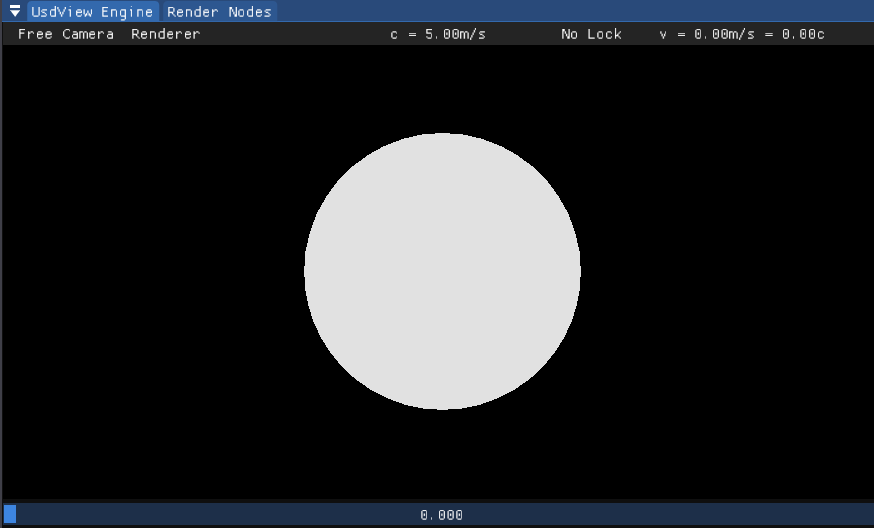
\includegraphics[width=\textwidth]{Camera.png}
        \caption{Camera Interface}
        \label{camera}
    \end{minipage}
\end{figure}

\subsubsection*{2.2 Key Relativistic Nodes}

\paragraph{1. Relativity Console}
The \textbf{Relativity Console} node (Figure \ref{console}) is provided in the \textbf{Composition} section to control fundamental parameters of the relativistic simulation. Controllable parameters include:

\begin{enumerate}[(1)]
    \item \textbf{Speed of light} (units: m/s).
    \item \textbf{Maximum camera velocity}, expressed as a fraction of the speed of light. Values close to or exceeding 1 are discouraged as they may produce unpredictable results.
    \item \textbf{Enable finite-speed-of-light transformations}: Recommended for activation to observe effects described in the principles or demonstrated in the results.
    \item \textbf{Newton iteration count}: Controls the number of iterations for solving delayed transformation effects and "god's eye" view computations. Higher values yield better accuracy at the cost of performance. Insufficient iterations may result in incorrect deformations and errors in meshes.
    \item \textbf{Damping for iterations}: To prevent explosive results during iterative calculations, apply a damping effect to iteration updates. If explosions occur, increase iteration count or reduce the damping coefficient.
    \item \textbf{Enable "god's eye" view}: Activate to simulate the god's eye perspective.
\end{enumerate}

\begin{figure}[htbp]
    \centering
    \setlength{\abovecaptionskip}{0.cm}
    \begin{minipage}[b]{0.3\linewidth}
        \centering
        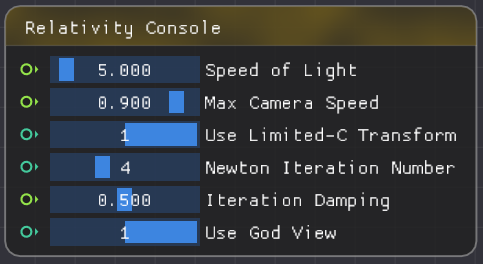
\includegraphics[width=\textwidth]{Console.png}
        \caption{Relativity Console}
        \label{console}
    \end{minipage}
    \quad
    \begin{minipage}[b]{0.5\linewidth}
        \centering
        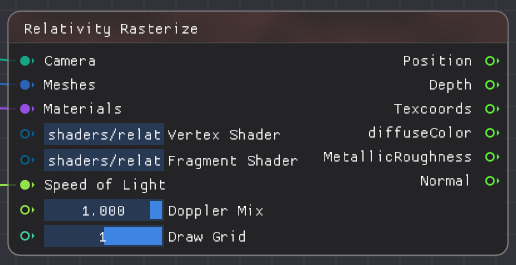
\includegraphics[width=\textwidth]{RelativityRasterize.png}
        \caption{Relativity Rasterize Node}
        \label{re_rasterize}
    \end{minipage}
\end{figure}

\paragraph{2. Relativity Rasterize Node}
In the Render node, the \textbf{Relativity Rasterize} node (Figure \ref{re_rasterize}) is provided with default relativistic shaders, including a Vertex Shader and a Fragment Shader. This rasterization incorporates relativistic wave vector transformations, accounting for changes in light direction and wavelength due to relativistic effects. However, it does not include delayed transformation effects caused by the finite speed of light. When using this node, be sure to enable \textbf{Use Limited-C Transform} in the Console to ensure accurate visual phenomena. Adjustable parameters include \textbf{Doppler Mix} and \textbf{Draw Grid}:
\begin{itemize}
    \item \textbf{Doppler Mix}: Ranges from $[0,1]$, where 0 ignores Doppler effects and 1 applies full Doppler effects. If Doppler effects become too intense, causing the spectrum to shift into infrared or ultraviolet (making it invisible), consider lowering the parameter, though this adjustment is not physically accurate.
    \item \textbf{Draw Grid}: Enables a grid on the xOy plane, which serves as a reference for observing object deformations.
\end{itemize}

\paragraph{3. Post-Processing Nodes}
As shown in Figure \ref{postprocess}, the Render node provides \textbf{Post Process} and \textbf{Mix Color} nodes. 
\begin{itemize}
    \item The \textbf{Post Process} node accepts information from the G-Buffer and passes it into shaders for post-processing effects such as SSAO, blur, and Bloom.
    \item The \textbf{Mix Color} node blends two texture images using blending modes defined in the shader and outputs the blended image. An example of post-processing is shown in Figure \ref{render} on page 16.
\end{itemize}

\begin{figure}[htbp]
    \centering
    \setlength{\abovecaptionskip}{0.cm}
    \begin{minipage}[b]{0.6\linewidth}
        \centering
        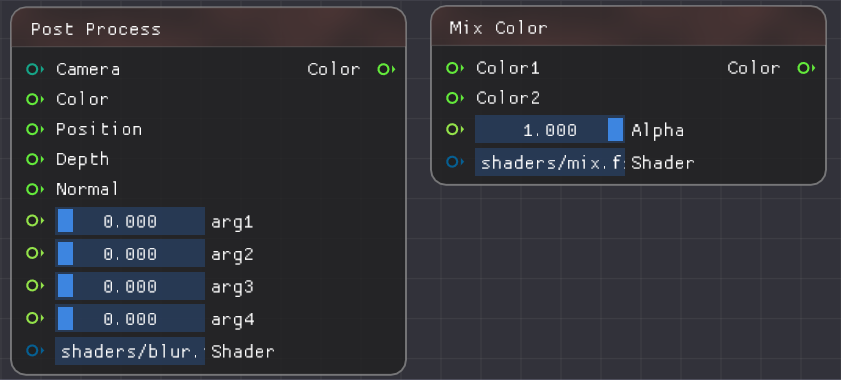
\includegraphics[width=\textwidth]{PostProcess.png}
        \caption{Post-process node}
        \label{postprocess}
    \end{minipage}
\end{figure}

For post-processing shaders:
\begin{itemize}
    \item \lstinline|blur.fs|: Implements Gaussian blur in a single direction.
    \item \lstinline|bilateral_filter.fs|: Performs bilateral filtering on textures.
    \item \lstinline|relativity_background.fs|: Renders the skybox for the main demonstration scene.
\end{itemize}

For blending mode shaders:
\begin{itemize}
    \item \lstinline|mix.fs|: Implements alpha blending ("normal").
    \item \lstinline|multiply.fs|: Implements multiply blending.
    \item \lstinline|add.fs|: Implements additive blending.
\end{itemize}

Node parameter usage:
\begin{enumerate}[(1)]
    \item The \textbf{Post Process} node provides four input parameters that can be passed to the shader. In the shader, the parameters can be accessed as follows:
\begin{lstlisting}[language=C++, title=Shader Input Parameters]
uniform float arg1;
uniform float arg2;
uniform float arg3;
uniform float arg4;
\end{lstlisting}
    \item The \textbf{Mix Color} node's Alpha parameter adjusts the blending ratio between two colors or serves other custom purposes.
\end{enumerate}

Note: These nodes are unrelated to relativistic visual effects themselves; they are designed for improved visual quality and ease of comparison.

\subsubsection*{Special Relativistic Visual Effects}
A node graph is shown in Figure \ref{view}. When using this setup:
\begin{enumerate}[(1)]
    \item Disable \textbf{Use God View} in the Console and connect the \textbf{Relativity Rasterize} node for rendering.
    \item Multiple methods are supported for importing objects: Read Usd imports (Geometric Nodes or Composition section), imports after animation processing, and imports of results from physical simulations. In the current code, only meshes output in Geometric Nodes with a \lstinline|Prim Path| of "geometry" in the \textbf{Write Usd} node can participate in delayed transformation calculations. 
    \item To enable delayed transformations for other imported moving objects or ensure all meshes participate, remove the following line (line 206) from \lstinline|RCore/hd_USTC_CG_GL/geometries/mesh.cpp|:
\begin{lstlisting}[language=C++, title=mesh.cpp, firstnumber=206]
    if (path == "/geom/geometry")
\end{lstlisting}
        Then recompile the program. Note that this may significantly increase performance costs for large models, such as \lstinline|Sponza_subdivided.usda|.
\end{enumerate}

\begin{figure}[htbp]
    \centering
    \setlength{\abovecaptionskip}{0.cm}
    \begin{minipage}[b]{0.85\linewidth}
        \centering
        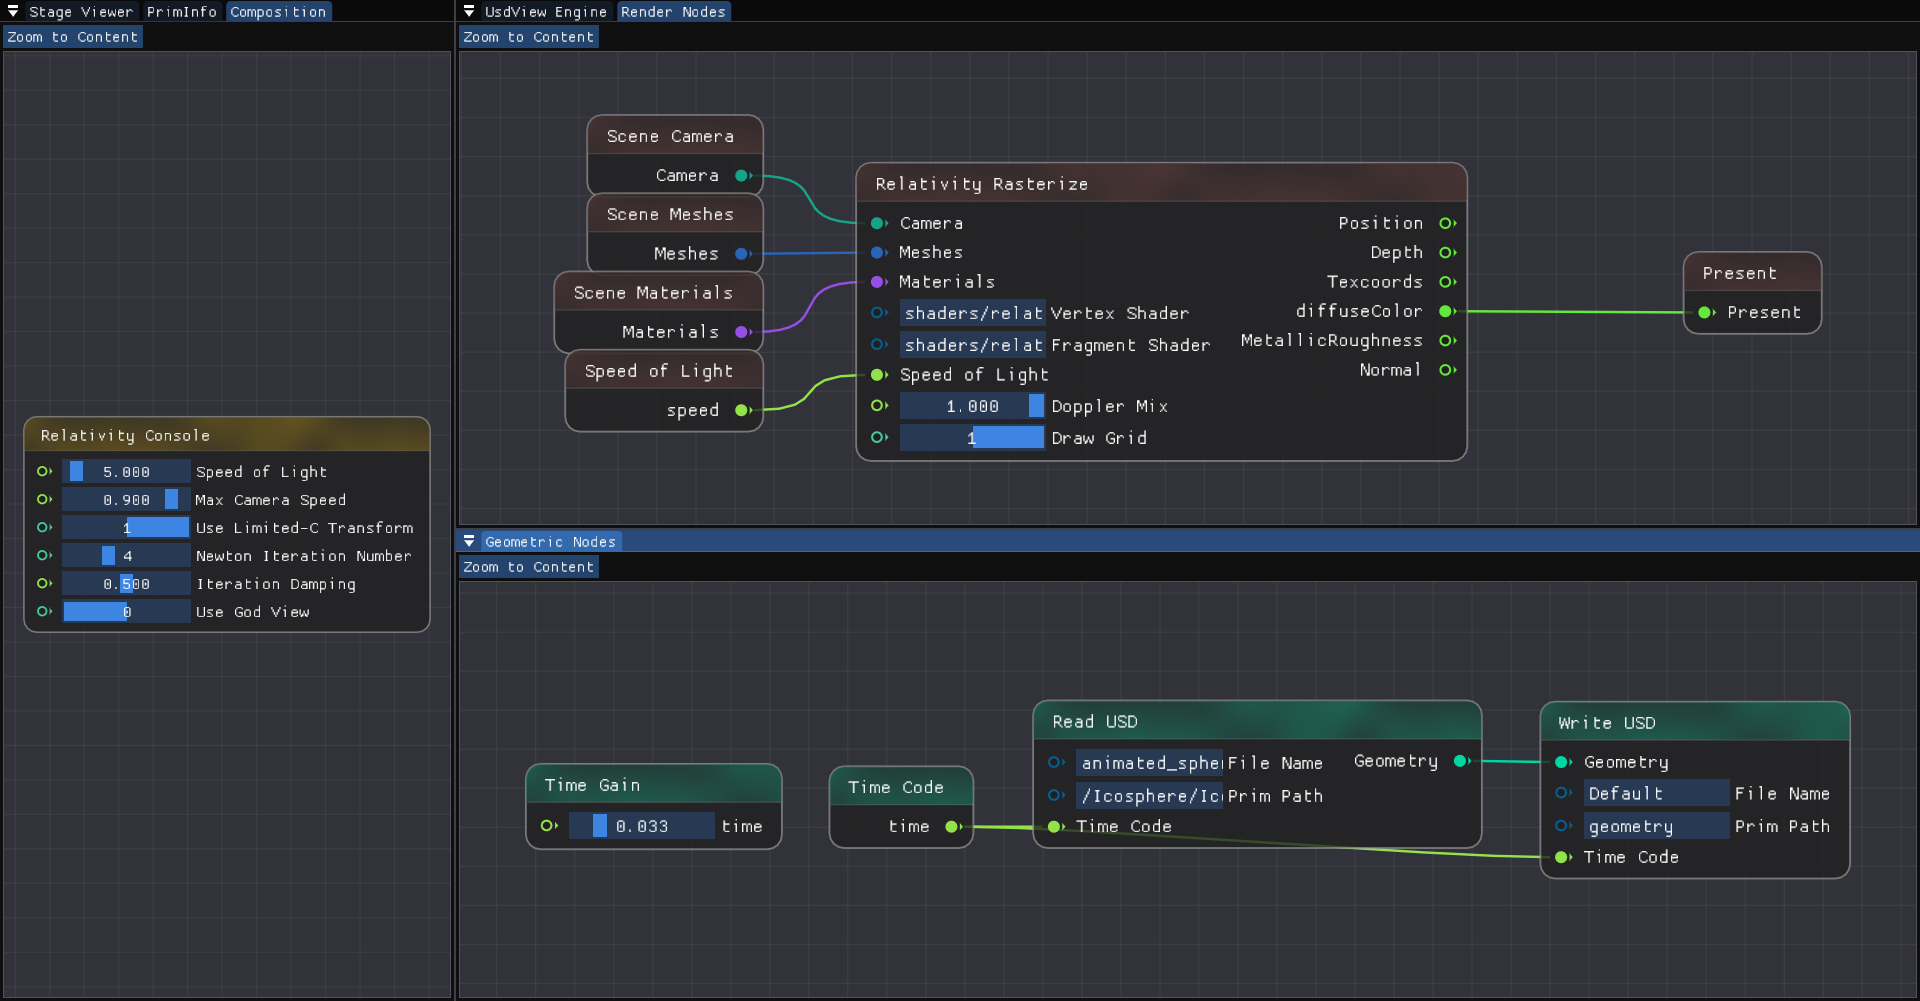
\includegraphics[width=\textwidth]{View.png}
        \caption{Special Relativistic Visual Effects Node Graph}
        \label{view}
    \end{minipage}
\end{figure}

\subsubsection*{God's Eye View Simulation}
A basic example of a "God's Eye View" simulation node graph is shown in Figure \ref{godview}. When using it:
\begin{enumerate}[(1)]
    \item Enable \textbf{Use God View} and do not use the \textbf{Relativity Rasterize} node (disregarding light propagation). Render meshes directly using standard rasterization methods.
    \item Run the simulation for the entire time range and save the meshes for all time steps before starting the God's Eye View simulation.
    \item Due to implementation details, all objects in the scene must be moving, and camera movement must occur while the \textbf{UsdView Engine} is playing to trigger the God's Eye View module.
\end{enumerate}

\begin{figure}[htbp]
    \centering
    \setlength{\abovecaptionskip}{0.cm}
    \begin{minipage}[b]{0.85\linewidth}
        \centering
        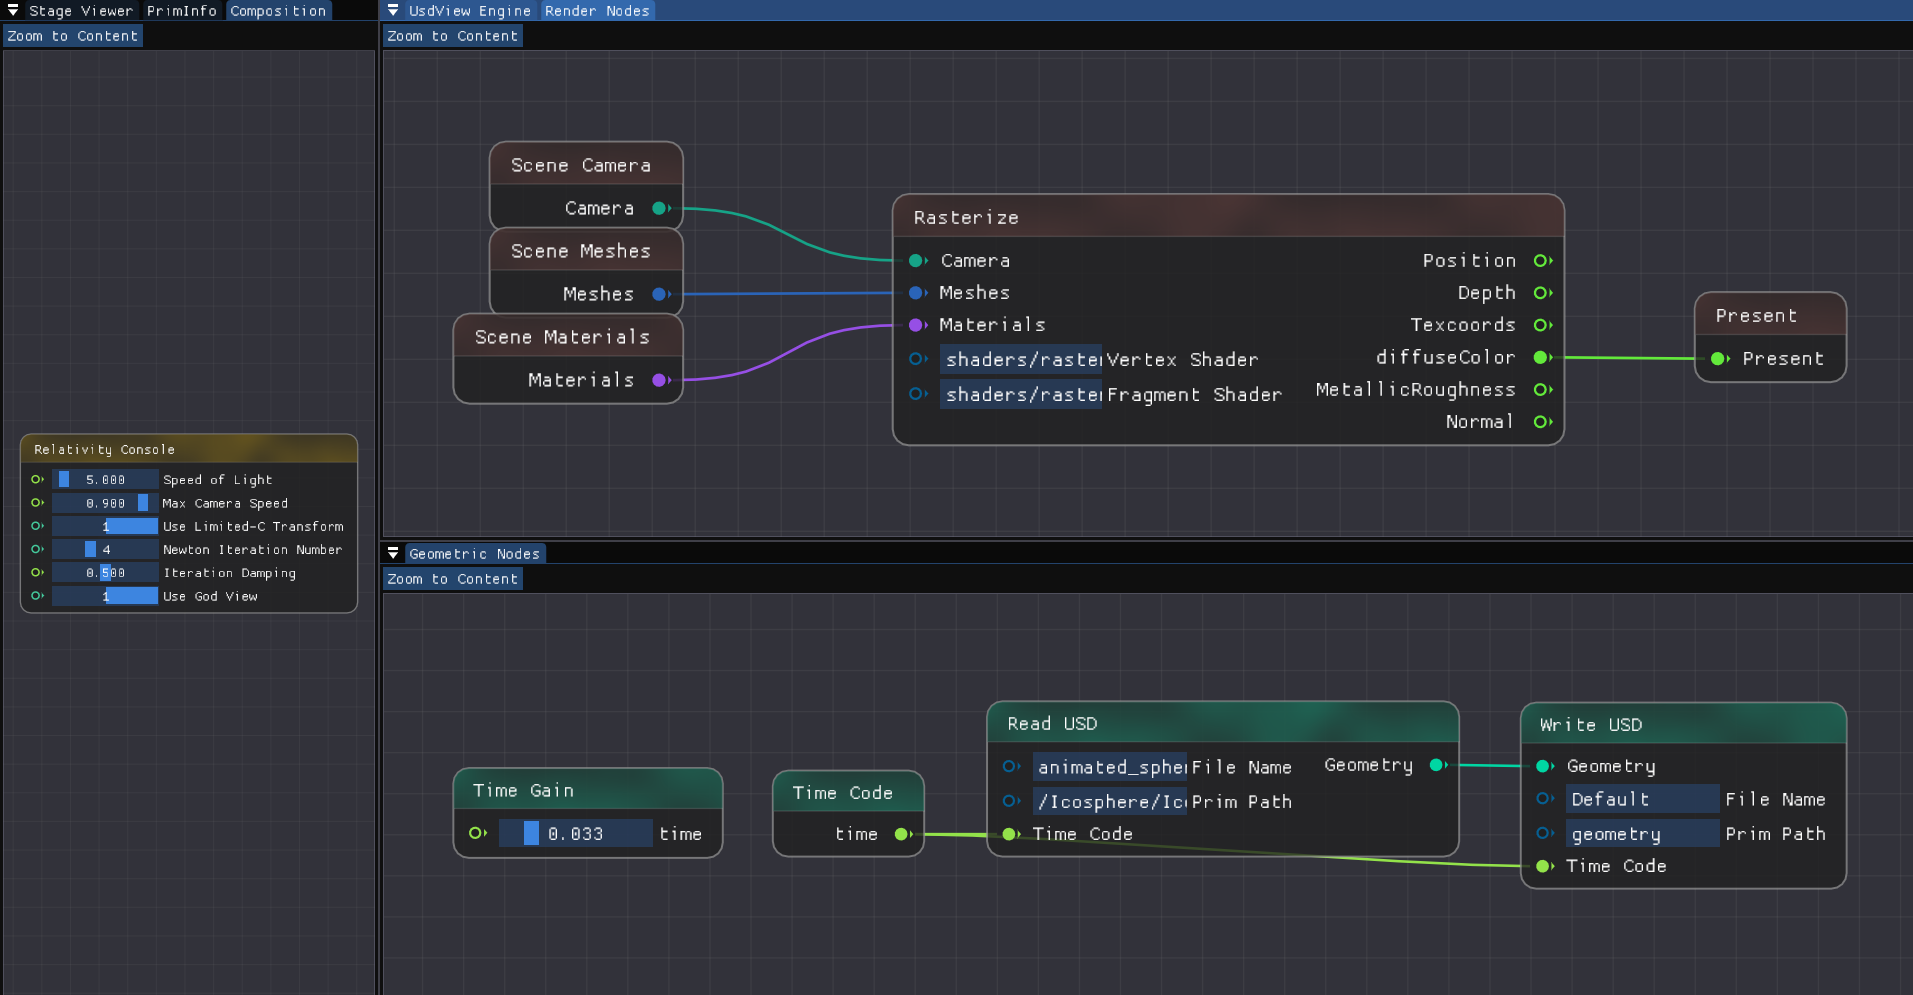
\includegraphics[width=\textwidth]{GodView.png}
        \caption{God's Eye View Simulation Node Graph}
        \label{godview}
    \end{minipage}
\end{figure}
\newpage

\subsubsection*{Special Relativistic Particle-Spring System Simulation}
Figure \ref{massspirng} shows a node graph for simulating a particle-spring system with collisions involving spheres (all within Geometric Nodes). The particle-spring calculation node is almost identical to that in Assignment 8, with added inputs for the speed of light and energy correction options (\lstinline|enable energy correction|). 
\begin{itemize}
    \item Setting this parameter to 0 disables corrections.
    \item Setting it to 1 applies tangent corrections.
    \item Setting it to 2 applies secant corrections (recommended). Detailed explanations are provided in the theory and implementation sections later in this document.
\end{itemize}

Simulation results are output to the \textbf{Write USD} node, representing the default frame of reference. Using the \textbf{Relativity Rasterize} or \textbf{God's Eye View} nodes, you can observe the simulation results from a relativistic perspective.

\begin{figure}[htbp]
    \centering
    \setlength{\abovecaptionskip}{0.cm}
    \begin{minipage}[b]{0.85\linewidth}
        \centering
        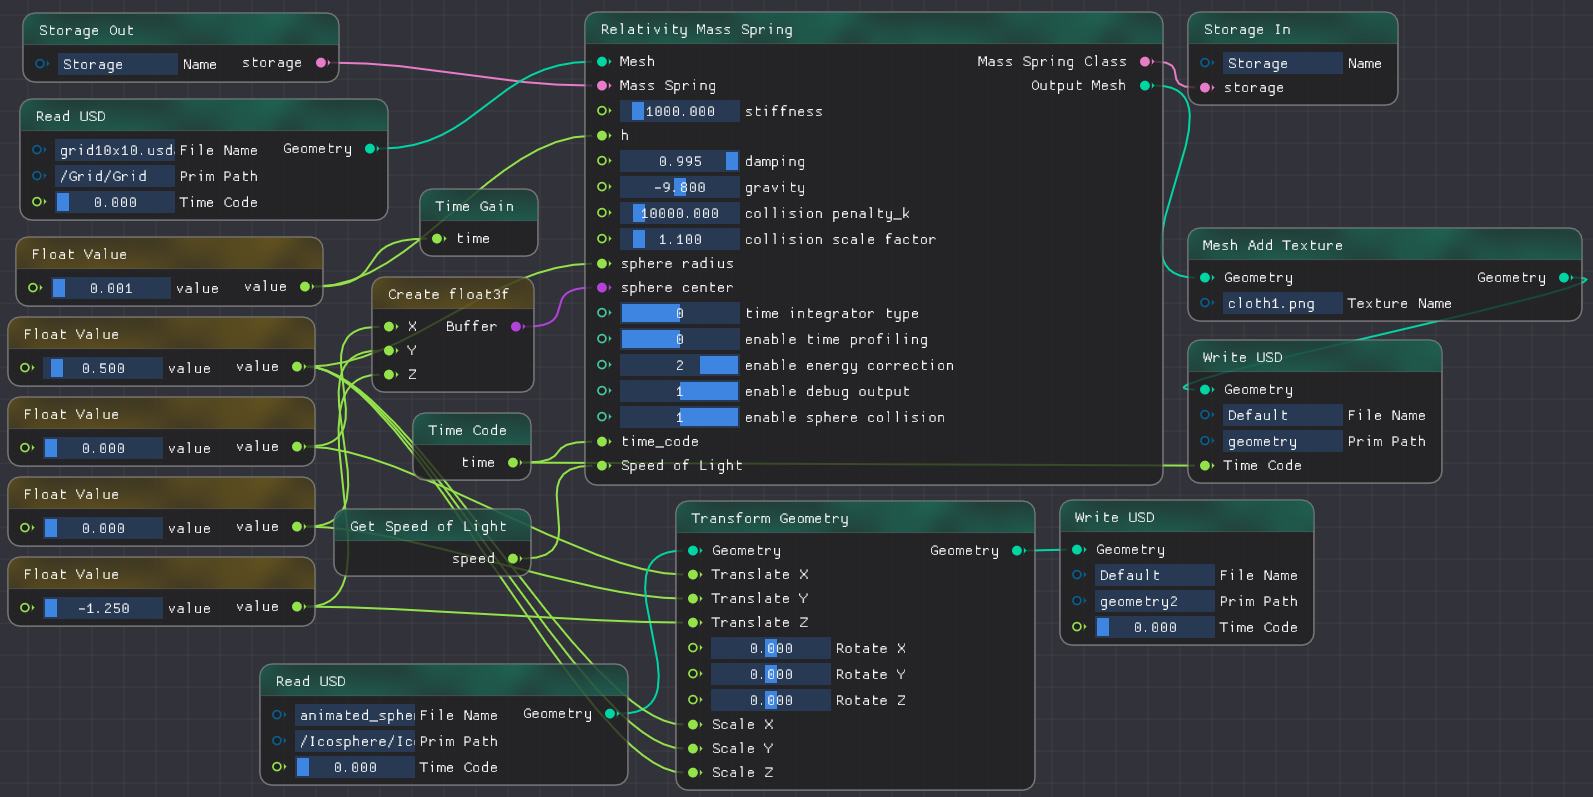
\includegraphics[width=\textwidth]{MassSpring.png}
        \caption{Special Relativistic Particle-Spring System Node Graph}
        \label{massspirng}
    \end{minipage}
\end{figure}

\newpage

\subsection*{3\quad Background, Principles, and Implementation}

\subsubsection*{Spacetime View in Special Relativity}

Newton's laws of motion are based on experimental results and summarize the motion of macroscopic, low-speed objects, with very broad applicability. Newtonian mechanics describes the motion of any object in inertial reference frames, and it satisfies the Galilean principle of relativity (the laws of mechanics have the same form in any inertial reference frame). The spacetime coordinates of the same physical event in two inertial reference frames follow Galilean transformations (velocity addition and time translation). However, some experiments have yielded different conclusions. Particle physics experiments show that as the energy of a particle increases, its velocity tends to a fixed value, which contradicts the energy calculations in Newtonian mechanics. Electromagnetism, developed from various electromagnetic experiments, is summarized in Maxwell's equations, which state that the speed of light in a vacuum is a constant $c = \frac{1}{\sqrt{\varepsilon_0 \mu_0}}$, which contradicts the linear velocity addition in Newtonian mechanics. Various new theoretical and experimental discoveries reveal contradictions that show that Newton's laws no longer apply to macroscopic, high-speed objects.

Einstein synthesized the various interpretations and attempts at resolving these contradictions and proposed the theory of special relativity. Special relativity assumes:
\begin{enumerate}[(1)]
    \item Space is homogeneous and isotropic, and time is homogeneous;
    \item The speed of light in a vacuum is the same for all observers, independent of the motion of the light source;
    \item The laws of physics have the same form in all inertial reference frames.
\end{enumerate}

We use four-dimensional coordinates to express spacetime positions. The inverse covariant spacetime coordinates (four-position) are defined as $x^{\alpha} = (x^{0}, x^{1}, x^{2}, x^{3}) = (ct, x, y, z)$, with the metric matrix in Minkowski space:
$$g_{\alpha \beta} = g^{\alpha \beta} = \begin{pmatrix} -1 & 0 & 0 & 0 \\ 0 & 1 & 0 & 0 \\ 0 & 0 & 1 & 0 \\ 0 & 0 & 0 & 1 \end{pmatrix}$$
The covariant spacetime coordinates are defined as $x_{\alpha} = g_{\alpha \beta} x^{\beta} = (-x^{0}, x^{1}, x^{2}, x^{3}) = (-ct, x, y, z)$. Under this metric, it can be proven that a general linear transformation between two inertial reference frames $x^{'} = \Lambda x + a$ (in four-dimensional form: $x^{'\alpha} = {\Lambda^{\alpha}}_{\beta} x^{\beta} + a^{\alpha}$) must satisfy $\Lambda^{\mathrm{T}} g \Lambda = g$ (or $\Lambda$ is an element of the Lorentz group $O(3,1)$, and such a transformation is called a Poincaré transformation). Without translation ($a = 0$), this becomes the Lorentz transformation. By considering infinitesimal Lorentz transformations, we can derive the Lorentz transformation that is independent of the choice of coordinate system:
$$ \begin{cases} ct^{'} = \gamma (ct - \vec{\beta} \cdot \vec{x}) \\ \vec{x}^{'}_{\parallel} = \gamma (\vec{x}_{\parallel} - \vec{\beta} ct) \\ \vec{x}^{'}_{\perp} = \vec{x}_{\perp} \end{cases} \quad \text{or} \quad \begin{cases} ct^{'} = \gamma (ct - \vec{\beta} \cdot \vec{x}) \\ \vec{x}^{'} = \vec{x} + \frac{\gamma^2} {\gamma + 1} (\vec{\beta} \cdot \vec{x}) \vec{\beta} - \gamma \vec{\beta} ct \end{cases} $$

Here, the primed coordinate system moves with velocity $\vec{v} = \vec{\beta} c$ relative to the unprimed system, where $\gamma = \frac{1} {\sqrt{1 - \beta^2}} \geq 1$. The subscript $_{\parallel}$ represents components parallel to the velocity, and $_{\perp}$ represents components perpendicular to the velocity (both are vectors). By reversing $\vec{\beta}$, we obtain the inverse transformation:
$$ \begin{cases} ct = \gamma (ct^{'} + \vec{\beta} \cdot \vec{x}^{'}) \\ \vec{x}_{\parallel} = \gamma (\vec{x}^{'}_{\parallel} + \vec{\beta} ct^{'}) \\ \vec{x}_{\perp} = \vec{x}^{'}_{\perp} \end{cases} \quad \text{or} \quad \begin{cases} ct = \gamma (ct^{'} + \vec{\beta} \cdot \vec{x}^{'}) \\ \vec{x} = \vec{x}^{'} + \frac{\gamma^2} {\gamma + 1} (\vec{\beta} \cdot \vec{x}^{'}) \vec{\beta} + \gamma \vec{\beta} ct^{'} \end{cases} $$

It can be proven that the direct and inverse transformations are consistent. Note that this transformation is invariant about the origin (when $t$, $t^{'}$, $\vec{x}$, and $\vec{x}^{'}$ are all 0, the transformation still holds), but in practice, this may not be the case, so the quantities should be understood as relative values or changes. The general matrix for a Lorentz transformation is:
$$ \Lambda = \begin{pmatrix} \gamma & -\gamma \vec{\beta} \\ -\gamma \vec{\beta} & \overleftrightarrow{I} + \frac{\gamma^2} {\gamma + 1} \vec{\beta} \vec{\beta} \end{pmatrix} $$
where $\overleftrightarrow{I}$ is the identity tensor.

The Lorentz transformation shows that the time and position of the same physical event may not be the same in different inertial reference frames, and they are related in a linear manner that depends on the relative velocity between the reference frames. This breaks the original simple spacetime view of Galilean transformations. An important difference is the relativity of simultaneity, which means that two events that happen simultaneously in one inertial reference frame may not occur simultaneously in another reference frame that is moving relative to the first. From the Lorentz transformation, we can derive two well-known effects in special relativity: time dilation and length contraction. Time dilation refers to the fact that for a uniformly moving object, if $\vec{x}^{'} = 0$, we have $t = \gamma t^{'}$, meaning that the time $t^{'}$ recorded by the moving object during its motion is shorter than the time $t$ recorded by a stationary observer. This occurs because the clocks are at different positions, and hence, from the perspective of the Lorentz transformation, time is different, reflecting the relativity of time intervals. Length contraction refers to the fact that for a ruler moving at a constant speed along its length direction, when the coordinates of both ends of the ruler are measured simultaneously in its own frame (i.e., $t^{'} = 0$), the length is $x^{'} = l_0$ (considering only motion in one dimension). In the stationary observer's frame, he must measure the length at the same moment ($t = 0$), and after applying the transformation, we get $x^{'} = \gamma x$, i.e., the measured length $l = x = \frac{l_0}{\gamma} < l_0$, which is shorter than the ruler's own length. This is because, in the stationary observer's frame, the two ends of the ruler are measured simultaneously, while in the moving ruler's frame, the measurement is not simultaneous, which results in the wrong length. This reflects the relativity of spatial intervals, and its essence is also the relativity of simultaneity.

\subsubsection*{More Transformations of Physical Quantities}

Based on the tools for describing Minkowski space and the general form of linear transformations, we can extend this to the transformations of other four-dimensional scalars, vectors, and tensors, resulting in the transformation formulas for many other physical quantities. Define the four-velocity $u^{\alpha} = \frac{\mathrm{d} x^{\alpha}} {\mathrm{d} \tau} = \gamma (c, \vec{v})$, where $\tau$ is the proper time (the time elapsed in the rest frame), then after transformation, the velocity addition rule in special relativity can be obtained as: 
$$ \begin{cases} 
\vec{\beta_{\parallel}} = \frac{\vec{\beta_{\parallel}^{'}} + \vec{\beta_0}} {1 + \beta_0 \beta_{\parallel}^{'}} \\
\vec{\beta_{\perp}} = \frac{\vec{\beta_{\perp}^{'}}} {\gamma (1 + \beta_0 \beta_{\parallel}^{'})} 
\end{cases} $$ 
This represents the velocity $\vec{\beta}$ of an object moving with velocity $\vec{\beta^{'}}$ in the inertial reference frame moving with velocity $\vec{\beta_0}$ relative to a rest frame, with $_{\parallel}$ denoting the component parallel to $\vec{\beta}$. 

Define the four-acceleration $w^{\alpha} = \frac{\mathrm{d} u^{\alpha}} {\mathrm{d} \tau} = (\gamma^4 \vec{\beta} \cdot \vec{a}, \gamma^4 \vec{a}_{\parallel} + \gamma^2 \vec{a}_{\perp})$. It can be shown that the relation between the acceleration $\vec{a}^{'}$ in the rest frame and the acceleration $\vec{a}$ observed by a stationary observer is:
$$ \begin{cases} 
\vec{a}_{\parallel} = \frac{\vec{a}^{'}_{\parallel}} {\gamma^3} \\
\vec{a}_{\perp} = \frac{\vec{a}^{'}_{\perp}} {\gamma^2} 
\end{cases} $$ 
The acceleration observed by the stationary observer is smaller than that observed in the rest frame. 

Define the four-momentum $p^{\alpha} = m u_{\alpha} = \gamma mc (1, \vec{\beta}) = (\frac{\epsilon}{c}, \vec{p})$, where the relativistic energy $\epsilon = \gamma mc^2 = \frac{mc^2} {\sqrt{1 - \beta^2}}$ and relativistic momentum $\vec{p} = \gamma m \vec{v} = \frac{m \vec{v}} {\sqrt{1 - \beta^2}}$, so $p^{\alpha} = (\frac{\epsilon}{c} , \vec{p})$. The photon energy is $\epsilon = c|\vec{p}|$, and its relativistic four-momentum vector is given by $p^{\alpha} = (|\vec{p}|, \vec{p})$. Using this form of four-momentum makes it a four-vector and ensures that in the low-speed case, it reverts to classical mechanics results. The electromagnetic field can also be expressed as a corresponding four-vector in a covariant form. 

In considering the wave equation, define the four-wavevector $k^{\alpha} = (\omega / c, \vec{k}) = \omega / c (1, \hat{k})$, where $\omega$ is the frequency and $\vec{k}$ is the three-dimensional wavevector. It can be shown that the four-wavevector is a four-vector, and the transformation of the wavevector is given by:
$$ \begin{cases} 
\omega^{'} = \gamma (\omega - c \vec{\beta} \cdot \vec{k}) \\
\vec{k}^{'}_{\parallel} = \gamma (\vec{k}_{\parallel} - \vec{\beta} \omega / c) \\
\vec{k}^{'}_{\perp} = \vec{k}_{\perp} 
\end{cases} \quad \text{or} \quad 
\begin{cases} 
\omega^{'} = \gamma (\omega - c \vec{\beta} \cdot \vec{k}) \\
\vec{k}^{'} = \vec{k} + \frac{\gamma^2} {\gamma + 1} (\vec{\beta} \cdot \vec{k}) \vec{\beta} - \gamma \vec{\beta} \omega / c 
\end{cases} $$
From the transformation of the wavevector, we can see that waves emitted from a moving source not only experience a frequency shift (Doppler shift) but also have their direction altered. When treating light as a wave, this means that the direction and frequency of the light will differ in different inertial reference frames, i.e., the color will change.

\subsubsection*{Visual Effects of Special Relativity}

Time dilation and length contraction are well-known effects of special relativity. However, if the speed of light decreases to a certain value, making it possible to visually observe the motion of relativistic objects (where $\beta$ is not far less than 1), can we observe the length contraction? The answer is no. This is because the effects discussed earlier use a "God's eye view," meaning we can directly observe the position of the object at a given moment. However, since the light emitted by the object takes time to travel to the eye or the camera, and involves the propagation of light, what we actually see is not the position of the object at the current moment, but the position of the object from some time ago. This means that the visual effects of objects under special relativity are not as simple as length contraction. We can implement these visual effects through the four-dimensional wave vector transformation discussed above. We assume the world space is a "default inertial reference frame" (default frame), and the camera moves within it, creating the corresponding visual effects.

In principle, visual effects mainly arise from changes in the direction and wavelength of light. The process centers around "light rays," and we can naturally try to simulate this using ray tracing. To render the image seen by the camera, light rays are emitted and first transformed into the default frame. Then, we calculate the intersection with the scene in the default frame. If the light ray hits an object, and the object is moving relative to the default frame, we need to transform to the object's own frame (based on the location where the light hits) and then perform BRDF sampling, randomly select the emission direction, and transform back to the default frame to continue the ray tracing process. The key difference from traditional ray tracing is that at each emission or reception, we need to transform into the object's own frame or the default frame, considering the frequency shift and directional changes. 

However, there is another source of visual effects: during the time the light travels from the object to the camera, the object moves. Therefore, the object we see should be located at the position it occupied at a previous time, requiring "delayed time" processing (as described below). The time to look back differs for different particles. Using ray tracing algorithms, the problem of determining the exact moment and the position of the object arises. This requires solving the entire grid's shape at that moment and recalculating the intersections (in four-dimensional space, as discussed below). This is a difficult problem and will predictably involve a large amount of computation. Based on this, we decide to use the rasterization pipeline to simulate the visual effects.

First, consider a stationary object in the default frame and its visual effect in the moving camera's own frame. From the ray tracing perspective, this involves bending the light ray and calculating the intersection with the object. From the rasterization perspective, we primarily consider the position of the object in space. We can assume that the object emits light rays directed towards the camera. These rays change direction in the camera frame, which is equivalent to the object moving to the corresponding angle in the camera frame. We can perform spatial transformations for each vertex in the mesh, i.e., in the Vertex Shader, by calculating the object's position in the camera reference frame using the camera's position, velocity, and other parameters. It can be derived that the new orientation of the object obtained using the ray tracing approach matches the position derived using Lorentz transformations, reflecting the consistency of relativistic transformations. Under this transformation, the occlusion relationships between objects remain physically valid. After transforming the vertices, we can determine the position of the object in the camera's frame. The transformation of the position vector relative to the camera is:
$$\vec{x}^{'} = \vec{x} + \frac{\gamma^2} {\gamma + 1} (\vec{\beta} \cdot \vec{x}) \vec{\beta} - \gamma |\vec{x}| \vec{\beta}$$
Subsequently, OpenGL rasterizes the new mesh, and we use Normal Mapping to compute the correct normals after the transformation of the vertex positions. In the Fragment Shader, we need to consider color changes because the image is rasterized into many pixels. For each pixel, we determine the wavelength change factor through the transformation:
$$\omega = \omega^{'} \gamma (1 + \vec{\beta} \cdot \hat{k}^{'})$$
$$\lambda^{'} = \lambda \gamma (1 + \vec{\beta} \cdot \hat{k}^{'})$$
Note that $\hat{k}^{'}$ is the direction vector of the light ray directed towards the camera in the camera's reference frame. Knowing the wavelength change factor, we need to determine the transformation method for the known $(r, g, b)$ colors. Further details will be provided later. This simulates the visual effects of a stationary object in the default frame.

Now, consider a moving object in the default frame and its visual effect in the camera's frame. We need to account for the fact that the light received by the camera at this moment was emitted by the object at an earlier time. In addition to considering changes in the wavelength and direction of the light, we also need to account for the time it takes for the light to propagate (both of which are direct consequences of the finite speed of light). For moving objects, we are actually seeing light that was emitted by the object in the past (e.g., the sunlight we see now actually left the Sun eight minutes ago).

The spacetime diagram can help us better understand special relativity. As shown in Figure \ref{4dspace}, we use a three-dimensional space to represent a four-dimensional vector, with the vertical axis representing time (actually $ct$, to maintain consistent units), and the plane perpendicular to it representing three-dimensional space. Since the speed of motion cannot exceed the speed of light, the time distance $c\Delta t$ must always be greater than the spatial distance $|\Delta \vec{x}|$. If we also consider the motion of light, we must have $c\Delta t = |\Delta \vec{x}|$, and the light emitted in all directions forms the "future light cone" surface in the diagram (this surface is actually three-dimensional, known as a hypersurface). Points inside the cone represent possible past events. Similarly, the motion of the origin in the past is inside the past light cone; the light reaching the origin must have passed through the past light cone. This indicates that any light reaching the camera at a time $t$ must lie on the "camera's past light cone." If a point on the object passes through a certain location at time $t^{*}$, the four-dimensional coordinate of this point lies exactly on the past light cone (as shown in Figure \ref{4dintersect}). The light emitted by this point at time $t^{*}$ can reach the camera at time $t$, forming an image of the object (the trajectory of a point on the object in four-dimensional space is called the worldline, and here it means the worldline of a point on the object intersects the camera's past light cone). Let the camera's four-dimensional coordinates be $(x, y, z, ct)$, then the point $(x^{*}, y^{*}, z^{*}, ct^{*})$ on the past/future light cone must satisfy $c|t^{*} - t| = \sqrt{(x^{*} - x)^2 + (y^{*} - y)^2 + (z^{*} - z)^2}$, where the spacetime interval is $\Delta s^2 = -c^2\Delta t^2 + \Delta x^2 + \Delta y^2 + \Delta z^2$. From the spacetime diagram, we can see that the spacetime interval between points inside the past/future light cone and the origin is less than zero, the interval for points on the cone is zero, and the interval for points outside the light cone is greater than zero. To make the subsequent equation solving easier, we rewrite it as $\Delta s = -c|\Delta t| + |\Delta \vec{r}|$ ($|\Delta \vec{r}| = \sqrt{\Delta x^2 + \Delta y^2 + \Delta z^2}$), which satisfies the conditions above. Since we see the object at an earlier time, in electrodynamics, $t^{*}$ is called the "retarded time."


\begin{figure}[htbp]
    \centering
    \setlength{\abovecaptionskip}{0.cm}
    \begin{minipage}[b]{0.5\linewidth}
        \centering
        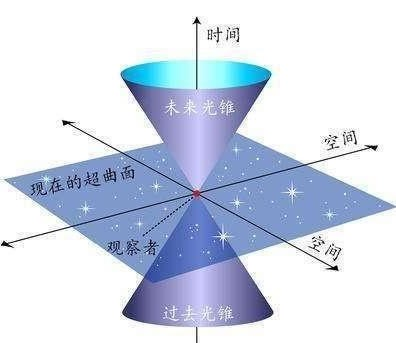
\includegraphics[width=0.8\textwidth]{4DSpace.jpeg}
        \caption{4D Space-Time diagram}
        \label{4dspace}
    \end{minipage}
    \begin{minipage}[b]{0.4\linewidth}
        \centering
        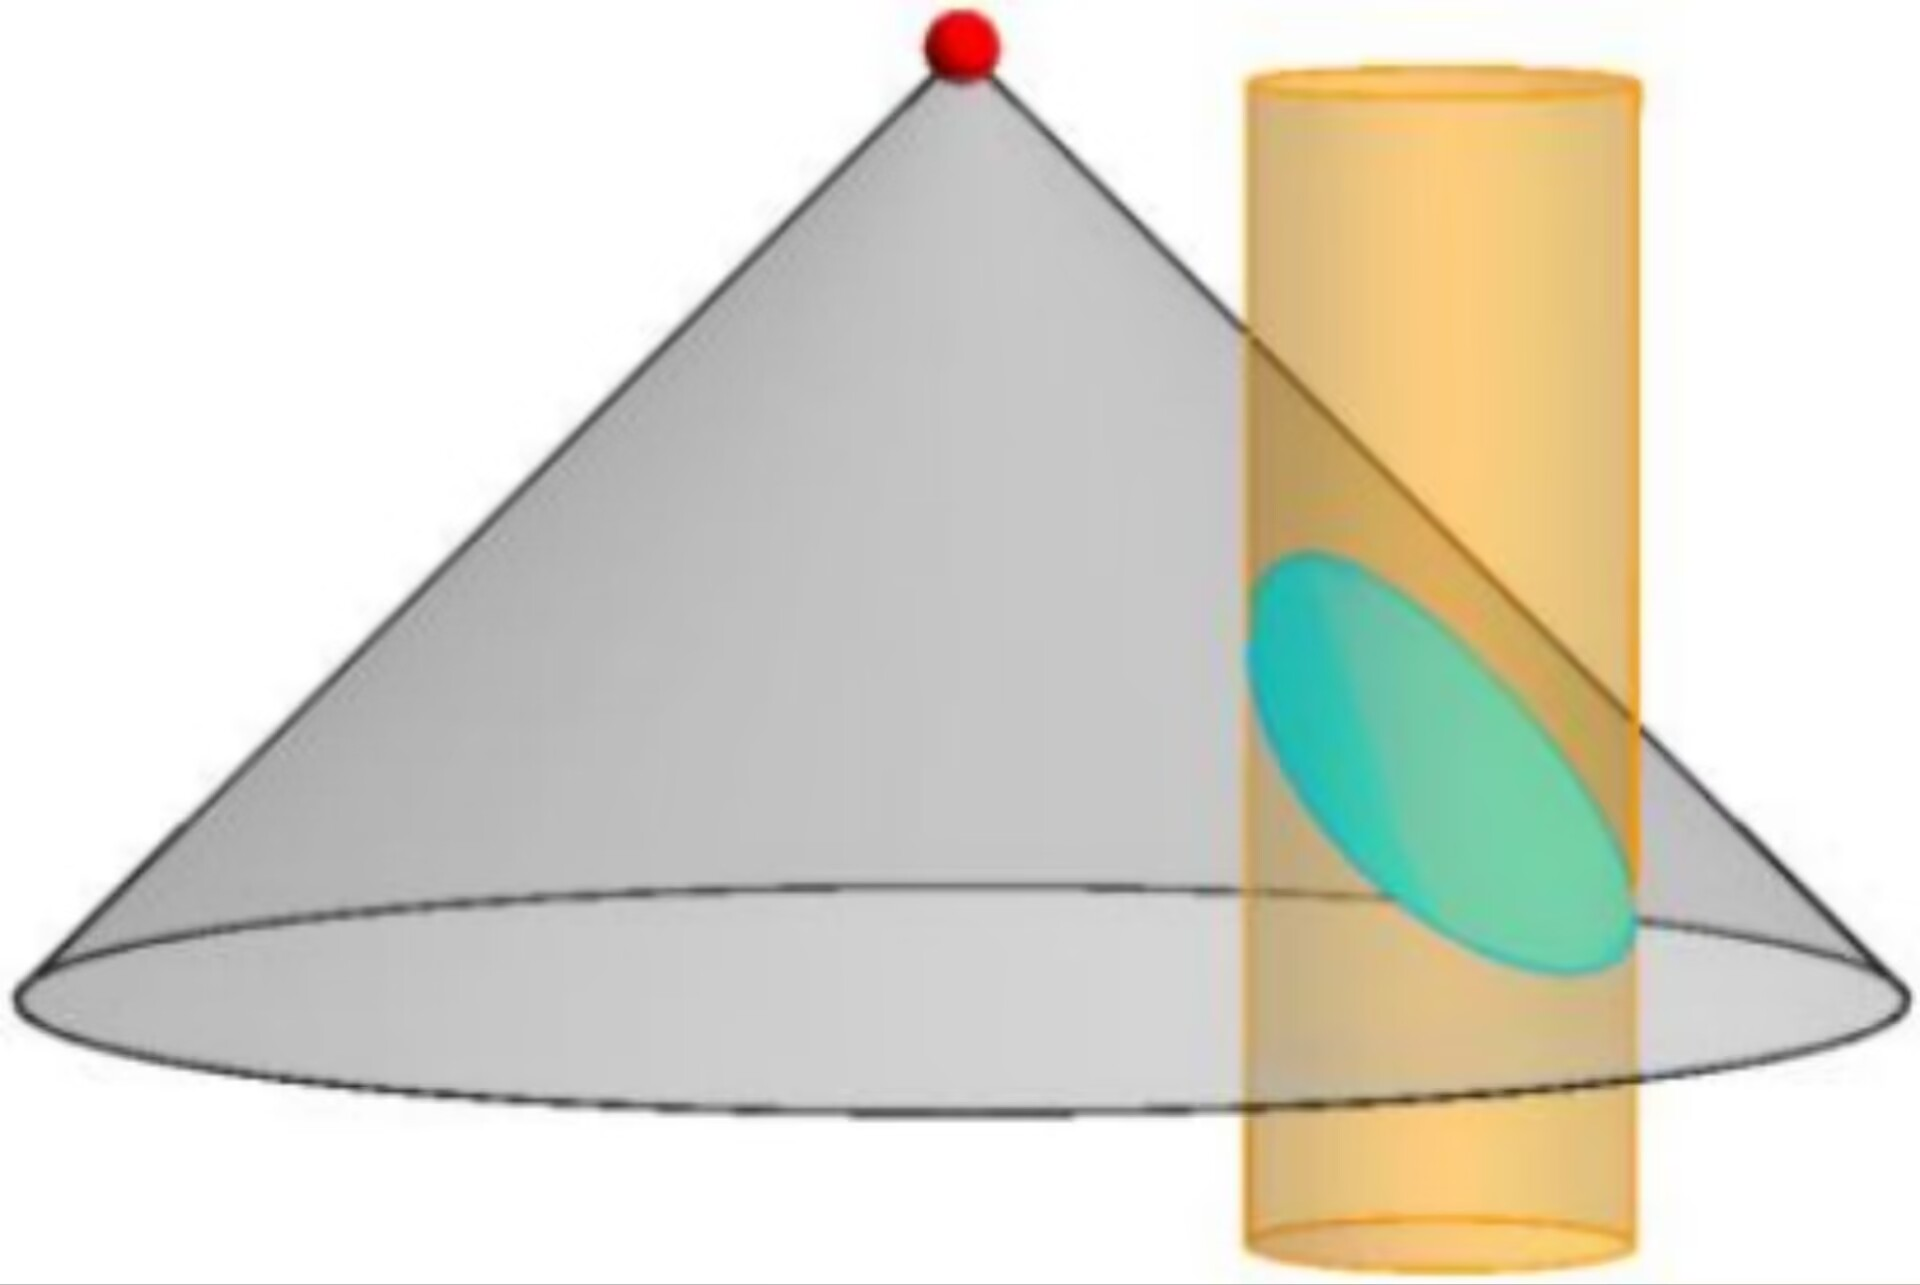
\includegraphics[width=0.8\textwidth]{4Dintersect.jpg}
        \caption{The past light cone intersects with the worldline, and the intersection plane is the actual three-dimensional grid seen}
        \label{4dintersect}
    \end{minipage}
\end{figure}

We know the position of a stationary object at any observation moment in the camera frame, because the object is stationary and does not involve "delayed time" processing. For moving objects, we need to obtain the trajectory of the object at each moment in time and solve the equation:
$$|\vec{x}(t^{*}) - \vec{x}_{\text{cam}}| = c(t - t^{*})$$
The required position of the object is $\vec{x}(t^{*})$. It should be noted that for physical scenes, the speed of the object must not exceed the speed of light. Therefore, the rate of change on the left side of the equation will not be greater than the right side. This is an equation of a monotonic function and can be solved using the bisection method or Newton's method. For situations where the speed of light is not too slow and the object's speed is not too fast, the derivative of the equation is relatively large, and Newton's method is more efficient. After solving for the new position of each vertex of the object, the situation becomes the same as that of a stationary object. We can proceed with steps such as rasterization and color computation. At this point, the color calculation uses the relative speed between the two as the reference frame for the speed. This simulates the visual effect of moving objects in the default reference frame. It is important to note that for moving objects, we need to recalculate the object's position during each rendering because the position of the camera changes over time.

\subsubsection*{Color Transformation}

We need to multiply the wavelength of the color by a factor, with the color represented in the form of $(r, g, b)$. To trace back to the wavelength, or the corresponding spectrum of the color, we need to refer to the definition of the sRGB color space (most Windows system devices operate in the sRGB color space when displaying general program content). As shown in Figure \ref{srgb} and Figure \ref{rgbcmf} (source: Wikipedia \url{https://en.wikipedia.org/wiki/CIE_1931_color_space}), the definition of RGB color values is as follows:
$$R = \int_{0}^{\infty} I(\lambda) r(\lambda) \mathrm{d} \lambda, \quad G = \int_{0}^{\infty} I(\lambda) g(\lambda) \mathrm{d} \lambda, \quad B = \int_{0}^{\infty} I(\lambda) b(\lambda) \mathrm{d} \lambda$$
where $I(\lambda)$ is the spectral power distribution. Here, we need to multiply the wavelength by a factor, which can be achieved by shifting $I(\lambda)$. Theoretically, changes in wavelength and direction may lead to changes in light intensity, but by ensuring energy conservation in a physical event over a given time period in a specified region, the height of the spectral power distribution should also change.

\begin{figure}[htbp]
    \centering
    \setlength{\abovecaptionskip}{0.cm}
    \begin{minipage}[b]{0.24\linewidth}
        \centering
        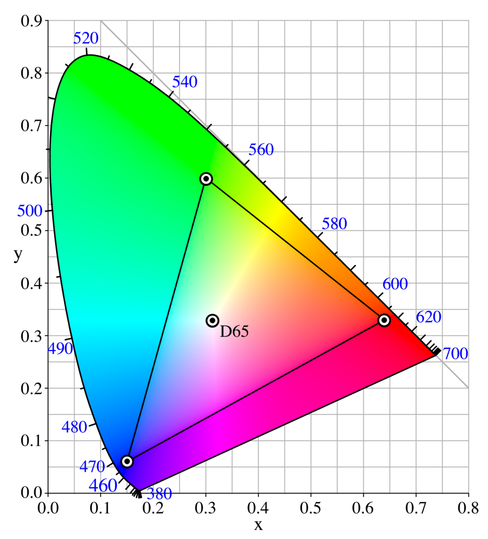
\includegraphics[width=\textwidth]{sRGB.png}
        \caption{RGB Primary Color Gamut}
        \label{srgb}
    \end{minipage}
    \begin{minipage}[b]{0.37\linewidth}
        \centering
        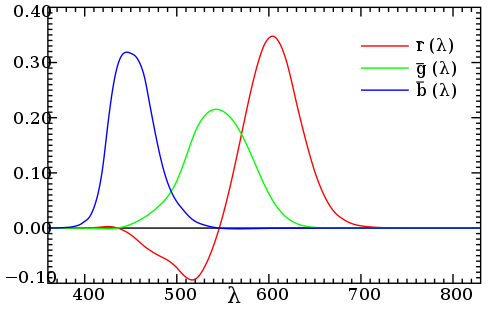
\includegraphics[width=\textwidth]{RGBCMF.png}
        \caption{RGB Color Matching Functions}
        \label{rgbcmf}
    \end{minipage}
    \begin{minipage}[b]{0.37\linewidth}
        \centering
        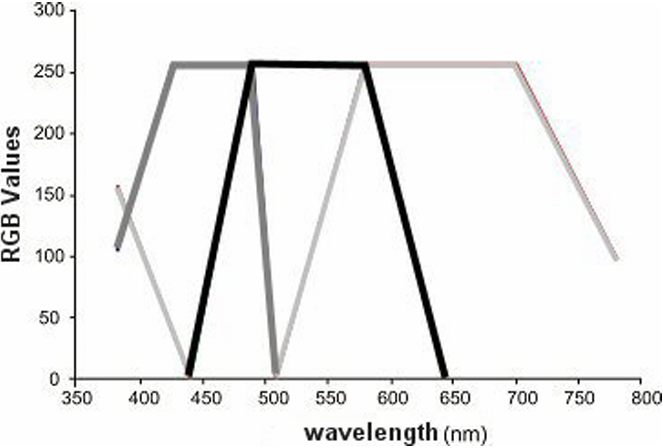
\includegraphics[width=\textwidth]{rgbsimp.png}
        \caption{Simplified RGB Color Matching Functions}
        \label{rgbsimp}
    \end{minipage}
\end{figure}

The above is the calculation method derived from the definition, which is highly accurate but computationally complex and requires a lot of prior knowledge, making it unsuitable for lightweight computational environments such as shaders. We attempt to simplify the color matching functions, as shown in Figure \ref{rgbsimp} (source: Miha, Dragos, and Eugen Strajescu. "FROM WAVELENGTH TO RGB FILTER." University Politehnica of Bucharest Scientific Bulletin, Series D: Mechanical Engineering 69.2 (2007): 77-84), simplifying it into a piecewise linear form, suitable for computation in shaders. At this point, each frequency corresponds to a specific color, using a linear, increasing attenuation, and gamma correction algorithm provided by Stack Overflow (source: \url{https://stackoverflow.com/questions/1472514/convert-light-frequency-to-rgb}). We first need to convert the given RGB color to the appropriate wavelength, perform the wavelength transformation, and then revert it to the color. From the curve, we can see that many RGB colors cannot be represented by a single wavelength. Here, we use a simplified approach, assuming that any RGB color is a linear combination of two wavelengths corresponding to two colors, with both intensity and color being linearly combined, and changing the wavelength does not affect the light intensity. We try to revert to two wavelengths that are close in color, as this is closer to the actual situation. In practice, especially when the speed of light is close to the motion speed, the wavelength can easily shift to the ultraviolet and infrared regions, causing the area to turn black and becoming difficult to observe. To achieve a better visual effect, we designed the parameter Doppler Mix to control the mixing ratio of the Doppler effect.

\subsubsection*{Camera Movement}

In this case, we use the original camera, set to accelerate and decelerate using the WASDQE keys, making the camera movement smoother. To ensure proper rendering, the camera's maximum speed is limited to the speed of light. The camera's speed is passed through \lstinline|renderParam| into the rendering \lstinline|Scene Camera| node from \lstinline|renderDelegate| via the \lstinline|SetRendererSetting| during each global GUI refresh of \lstinline|usdview_engine|, allowing it to be utilized by the rendering node and Shader.

In theory, similar to Newtonian mechanics, the framework of special relativity is still only applicable to inertial reference frames. However, the camera’s motion cannot be without acceleration, and thus it is not an inertial reference frame. Our solution to this is to use a “snap reference frame”—an inertial reference frame that moves with the same velocity as the camera at that moment—for transformations and rendering. The validity of this approach can be considered from the perspective of four-dimensional spacetime worldlines. Considering that physical velocities do not change abruptly, the transformation of light is also continuous, and the scene changes continuously. In the current discrete time rendering, using smooth camera motion helps achieve more continuous rendering results and a better visual experience. Additionally, based on Lorentz transformation, in the camera’s reference frame, after a time interval of $\Delta t$, the default reference frame should have passed $\gamma \Delta t$ time. When observed in the camera reference frame, the operating system time is not the same as the time passed in the default reference frame. However, achieving this in the current framework is quite difficult, so for now, we treat time in both reference frames as the same. This compromise has little impact on visual effects but may affect the motion behavior.

\subsubsection*{Implementation of Delayed Time}

In order to solve the function $f(t^{*})=|\vec{x}(t^{*}) - \vec{x}_{\text{cam}}| - c(t - t^{*})$ for the zero point at each vertex in every frame using Newton's method, we need to access $f(t^{*})$ values at each time step with low overhead. To transform the vertices before rasterization, we investigated the framework's operation and decided to implement vertex transformation in the update vertex function called for each Mesh in the rasterization, specifically in \lstinline|RCore/hd_USTC_CG_GL/geometries/mesh.cpp| in the \lstinline|Hd_USTC_CG_Mesh::Sync| function.

After passing the Global Usd Stage pointer, which stores the object positions at each timestamp, from \lstinline|usdview_engine.cpp| to Render Params, we can access this data in the \lstinline|Sync()| function. The obtained data is discrete, and to get the value of $f(t^{*})$ at any given $t^{*}$, we need to interpolate the function. The framework itself provides functionality for discrete position interpolation, but due to implementation constraints, each interpolation call would require interpolating all vertices in the Mesh, which is computationally expensive. Therefore, we manually implemented linear interpolation for object positions.

Specifically, we first obtain the list of stored Time Samples. When we need to compute the vertex position at $t^{*}$, we use the \lstinline|std::lower_bound| function from the STL to find the largest lower bound of $t^{*}$ in the timestamp list and further calculate the smallest upper bound. After obtaining the position information for the two closest timestamps, we assume the vertex moves at a constant velocity in this time interval, using linear interpolation to compute the position at $t^{*}$ and directly calculate the velocity. For cases where $t<0$, we assume the object is stationary to calculate the vertex position.

Differentiating, we get $f'(t^{*})=\dfrac{(\vec x - \vec x_{\text{cam}})}{|\vec x - \vec x_{\text{cam}}|} \cdot \vec v+c$. Using Newton's method, $t_{n+1}^{*}=t_{n}^{*}-k\dfrac{f(t_{n}^{*})}{f'(t_{n}^{*})}$, we can calculate the reasonable new position of the vertex after several iterations. Here, $0<k \le 1$ is a constant (also known as Iteration damping), generally set to 1 but can be reasonably adjusted to ensure iteration stability.

It is also important to note that the principle of 3D animation is usually to apply a Transform to the entire model rather than record the position of each vertex at each timestamp. This implementation needs to modify the position of each vertex, rather than applying the same Transform to the entire object. Therefore, when reading the vertex positions at each timestamp, the transformation is applied to the vertices, and the new position is calculated in world coordinates, with the identity matrix passed as the Transform to the rasterization vertex.

\subsubsection*{Simulation from the God’s Eye View}

In addition to visual effects, we also retain simulations of classic relativistic phenomena (e.g., length contraction), which reflect relativistic effects in traditional views. In this view, the propagation of light is ignored, and what we "see" at a specific moment $t_0$ is considered as a slice of four-dimensional space at $t=t_0$. For example, when we say "an object exists at a certain place at $t=t_0$" instead of "we saw an object," we disregard the light propagation required for visual perception. Accordingly, we only need to find all points at the moment $t=t_0$ to construct a three-dimensional space from the God’s eye perspective. Since the camera reference frame moves relative to the default frame, the points seen by the camera should form a set at $t' = t_0'$. Assuming that at the point of the camera $t=t'$ (as mentioned above, ignoring time dilation differences between the camera in the two reference frames), and the camera’s position in the default reference frame transforms to the camera’s position in the camera frame, the "four-dimensional vector relative to the camera's four-dimensional coordinates" satisfies the Lorentz transformation. Since the camera can see its own "moment," we say that the relative four-dimensional vector of things in space at that moment must satisfy $\Delta t' = 0$. According to the formula, the equation that this point satisfies is $c\Delta t - \vec{\beta} \cdot \Delta \vec{x} = 0$. Taking the derivative with respect to $\Delta t$, we get $c - \vec{\beta} \cdot \vec{v}$ (the camera’s speed and the time interval (the derivative can only depend on the time $t$ of the point in the default frame, so no other terms are included)), which is greater than zero, indicating that the left-hand side of the equation is a monotonically increasing function, so it must have a unique solution.

The solution method is the same as in the previous section, using Newton’s method for iteration. However, there are some differences:
\begin{enumerate}[(1)]
    \item The delayed time is always less than the real time, but here $\Delta t$ has no positive or negative restriction. Therefore, the correct God’s eye view solution requires first calculating the grid for all moments in the default reference frame. From a practical point of view, this means running the simulation once to ensure that the GeomMesh in the Global Usd Stage contains all valid mesh information from moments 0 to 250, and then performing the God’s eye view simulation.
    \item The solution for $t$ is likely to be less than 0 or greater than 250. By searching Time Samples, the result assumes that the object is stationary at $t < 0$ and $t > 250$, and that its motion is continuous. This way, the worldline is extended to $(-\infty, +\infty)$, ensuring a unique solution for the equation. Avoiding the approximation of an object "appearing and disappearing" greatly improves the feasibility and simplicity of achieving relativistic visual effects. If an object involves appearing at a certain moment and disappearing at another, due to simultaneity in relativity, two different points on the object are simultaneous in the default frame but not in the camera frame. Therefore, the mesh seen at that moment should be incomplete (this also applies to delayed time calculations). This requires deleting points from the mesh, and if the mesh is not fine enough, interpolation may be necessary in some places to modify its topological structure. Assuming that objects do not appear and disappear effectively avoids these operations.
    \item Since the following steps directly connect to the Rasterize node, we need to perform Lorentz transformation on the results here. The transformation vector form is $\Delta \vec{x}' = \Delta \vec{x} + \frac{\gamma^2}{\gamma + 1} (\vec{\beta} \cdot \Delta \vec{x}) \vec{\beta} - \gamma \vec{\beta} c \Delta t$, which is implemented in the code. By substituting into the equation $c \Delta t - \vec{\beta} \cdot \Delta \vec{x} = 0$, we can simplify it to $\Delta \vec{x}' = \Delta \vec{x} - \frac{\gamma}{\gamma + 1} (\vec{\beta} \cdot \Delta \vec{x}) \vec{\beta}$. It can be observed that if $\vec{\beta}$ becomes $-\vec{\beta}$, the result $\Delta \vec{x'}$ does not change! This also explains the phenomenon in the video where similar scenes are observed when moving forwards and backwards.
\end{enumerate}

\subsubsection*{Special Relativity Physics Simulation}

The spacetime view of special relativity discussed above solves the kinematic problems of objects in special relativity, but it does not provide a solution for the dynamics. Based on the idea that the motion laws should align with Newton's laws of motion as the speed approaches the speed of light, the kinematic equations of motion for an object in special relativity can be derived:
$$\frac{\mathrm{d} \vec{p}} {\mathrm{d} t} = \vec{F}$$
which is consistent with Newton's second law in the form of momentum, but here momentum is represented by the relativistic momentum $\vec{p} = \gamma m \vec{v}$. Alternatively, it can be written in covariant form as $\frac{\mathrm{d} p^{\alpha}} {\mathrm{d} \tau} = K^{\alpha}$, where $K^{\alpha}$ is the four-force, and the four-momentum is as described above. If the form of the force is known, the motion of the object can be described using momentum, or more directly, the three-dimensional equations of motion can be written as:
$$ \begin{cases} \gamma^3 m \vec{a}_{\parallel} = \vec{F}_{\parallel} \\ \gamma m \vec{a}_{\perp} = \vec{F}_{\perp} \end{cases} \quad \text{or} \quad \gamma m \vec{a} = \vec{F} - (\vec{\beta} \cdot \vec{F}) \vec{\beta}, \vec{a} = \frac{1} {\gamma m} (\vec{F} - (\vec{F} \cdot \vec{\beta}) \vec{\beta})$$
This equation is valid in any inertial frame. Here, $\vec{\beta}$ represents the velocity of the particle, so for relativistic physics simulations, we only need to use the above equations in the default frame without considering Lorentz transformations. These are the fundamentals of relativistic physics simulations.

Consider the simulation of a particle-spring system (Mass Spring), with principles and derivations referenced in Homework 8. The particle-spring system assumes point masses with no volume, connected by light ideal springs, which simulate the motion of fabric. In the relativistic case, we still assume that the forces acting on the objects remain unchanged: gravity is the average effect of space-time gravitational forces, rotation, etc., and can be set to an appropriate value; the linear elastic force follows the experimental laws of real springs within the elastic limits, and thus, in the relativistic case, the form of the force should remain unchanged within the elastic limits.

The simplest semi-implicit method directly calculates the force and acceleration to obtain the velocity at the next time step, updating the position using the new velocity. For the relativistic case, the velocity update equation is modified as follows:
$$\vec{v}_{n+1} = \vec{v}_n + \vec{a} \Delta t = \vec{v}_n + h \cdot \frac{1} {\gamma} (\frac{\vec{F}} {m} - \frac{\vec{F}} {m} \cdot \vec{\beta} \vec{\beta})$$

In the implicit method, the next positions and velocities are solved for, forming the equations:
$$ \begin{cases} \vec{x}^{n+1} = \vec{x}^{n} + h \vec{v}^{n+1} \\ \vec{v}^{n+1} = \vec{v}^{n} + \frac{h}{\gamma} (\mathbf{I} - \vec{\beta} \vec{\beta}^\top) \cdot \mathbf{M}^{-1} (\vec{f} _ {\text{int}}(\vec{x}^{n+1}) + \vec{f}_{\text{ext}} ) \end{cases} $$
where $\mathbf{M} = m \mathbf{I}$. Thus, $ \vec{x}^{n+1} = \vec{x}^{n} + h \vec{v}^{n} + \frac{h^2}{\gamma} (\mathbf{I} - \vec{\beta} \vec{\beta}^\top) \mathbf{M}^{-1} (-\nabla E(\vec{x}^{n+1}) + \vec{f}_{\text{ext}} ) $, and define $\vec{y} = \vec{x}^n + h \vec{v}^n + \frac{h^2}{\gamma} (\mathbf{I} - \vec{\beta} \vec{\beta}^\top) \cdot \mathbf{M}^{-1} \vec{f}_{\text{ext}}$. The equation becomes:
$$ \frac{\gamma}{h^2} \mathbf{M} (\vec{x}^{n+1} - \vec{y}) + (\mathbf{I} - \vec{\beta} \vec{\beta}^\top) \cdot \nabla E(\vec{x}^{n+1}) = 0 $$
The original method transforms this equation into a gradient-zero equation, thereby converting it into a minimization problem of an energy function, which is solved using optimization methods. We need to examine if the equation can be transformed into a gradient form. This can be determined by checking if the divergence of the gradient is zero. Since $\mathbf{I} - \vec{\beta} \vec{\beta}^\top$ does not depend on the coordinates (here, $\vec{v}_n$ is used for calculation and not strictly implicit, otherwise nonlinear, which is harder to handle), it does not participate in the $\nabla$ operation. Let $\vec{x} = \vec{x}^{n+1} \in \mathbf{R}^{3n \times 1}$, and check whether $\nabla E(\vec{x}) \cdot \vec{\beta} \vec{\beta}$ is curl-free:
$$\nabla \times (\nabla E(\vec{x}) \cdot \vec{\beta} \vec{\beta}) = \nabla (\nabla E(\vec{x}) \cdot \vec{\beta}) \times \vec{\beta} = \vec{\beta} \cdot \nabla (\nabla E(\vec{x})) \times \vec{\beta}$$
The energy of the spring is $E = \sum \frac{1}{2} k (||\vec{x} - \vec{y}|| - L)^2$, $\nabla E = \sum k (\vec{x} - \vec{y}) (1 - \frac{L} {||\vec{x} - \vec{y}||} )$
$$\nabla (\nabla E) = \sum k (\mathbf{I} - \frac{L} {||\vec{x} - \vec{y}||^3} (||\vec{x} - \vec{y}||^2 \mathbf{I} - (\vec{x} - \vec{y}) (\vec{x} - \vec{y})^\top))$$
Also, $\vec{\beta} \cdot \mathbf{I} \times \vec{\beta} = \vec{\beta} \times \vec{\beta} = \vec{0}$. Thus,
$$\vec{\beta} \cdot \nabla (\nabla E(\vec{x})) \times \vec{\beta} = \sum kL \vec{\beta} \cdot \frac{(\vec{x} - \vec{y}) (\vec{x} - \vec{y})^T}{||\vec{x} - \vec{y}||^3} \times \vec{\beta}$$
which is not necessarily zero. The original vector equation cannot be converted into a gradient equation and thus cannot be transformed into a minimization of the energy function. Therefore, the original optimization method cannot be applied.

If the incorrectness at this point is ignored and the previous approach is continued, assume there exists a minimization function $\min_{\vec{x}} g(\vec{x})$, where
$$ \nabla g(\vec{x}) = \frac{\gamma}{h^2} \mathbf{M}(\vec{x} - \vec{y}) + (\mathbf{I} - \vec{\beta} \vec{\beta}^\top) \nabla E(\vec{x}) $$
Perform one Newton iteration: $ \vec{x}^{n+1} = \vec{x}^n - (\nabla^2 g)^{-1} \nabla g $, where
$$ \nabla^2 g = \frac{\gamma}{h^2} \mathbf{M} + (\mathbf{I} - \vec{\beta} \vec{\beta}^\top) \nabla^2 E(\vec{x}) $$
Using the same method to compute the Hessian matrix, we get $ \nabla^2 g = \frac{\gamma}{h^2} \mathbf{M} + (\mathbf{I} - \vec{\beta} \vec{\beta}^\top) \mathbf{H} $, noting that $\gamma$ and $\mathbf{I} - \vec{\beta} \vec{\beta}^\top$ are different for each vertex and should be processed separately.
Thus, 
$$ \vec{x}^{n+1} = \vec{x}^n - (\nabla^2 g)^{-1} \nabla g (\vec{x}^n) = \vec{x}^n + \Delta \vec{x}, $$
and the system of equations is:
$$ \nabla^2 g \Delta \vec{x} = -\nabla g $$
Solving this system will give the displacement, thus determining the position and velocity at the next time step.

The acceleration method uses the Local-Global optimization method, which requires $g$, but this does not exist. However, if we proceed step-by-step: first perform the Local Step: $ \vec{d}_i = L_i \frac{\vec{x}_i}{\|\vec{x}_i \|} $. Then consider the Global Step, which is also in gradient form:
$$ \nabla g(\vec{x}) = \frac{\gamma}{h^2} \mathbf{M}(\vec{x} - \vec{y}) + (\mathbf{I} - \vec{\beta} \vec{\beta}^\top) \nabla E(\vec{x}) $$
where $E = \frac{1}{2} \vec{x}^\top \mathbf{L}\vec{x} - \vec{x}^\top \mathbf{J} \vec{d} $, and $\nabla E = \mathbf{L} \vec{x} - \mathbf{J} \vec{d}$, with 
$$ \mathbf{L}=\left(\sum_{i=1}^s k_i \vec{A} _ i \vec{A} _ i^{\top}\right) \otimes \mathbf{I} _ 3, \quad \mathbf{J}=\left(\sum_{i=1}^s k_i \vec{A}_i \vec{S}_i^{\top}\right) \otimes \mathbf{I}_3, $$
$$ (\vec{A}_i)_j = 1 (\text{if the left end of spring i is j}), -1 (\text{if the right end of spring i is j}), 0 (\text{otherwise}) $$
and
$$ (\vec{S}_i)_j = 1 (i = j), 0 (i \neq j). $$
Therefore, the equation to solve is:
$$ \gamma \mathbf{M}(\vec{x} - \vec{y}) + h^2 (\mathbf{I} - \vec{\beta} \vec{\beta}^\top) (\mathbf{L} \vec{x} - \mathbf{J} \vec{d}) = 0 $$
$$ (\gamma \mathbf{M} + h^2 (\mathbf{I} - \vec{\beta} \vec{\beta}^\top) \mathbf{L}) \vec{x} = \gamma \mathbf{M} \vec{y} + h^2 (\mathbf{I} - \vec{\beta} \vec{\beta}^\top) \mathbf{J} \vec{d} $$
Solving this equation will give the new positions of all the points. For fixed points, it is best to handle them using a projection matrix: $\vec{x}^{'} = \mathbf{K} \vec{x}$, $\vec{x} = \mathbf{K}^{T} \vec{x}^{'} + \vec{b}$, where $\mathbf{K}$ is for dimension reduction, $\mathbf{K}^{T}$ for dimension expansion, and $\vec{b}$ represents the fixed points. Thus,
$$ \mathbf{K} (\gamma \mathbf{M} + h^2 (\mathbf{I} - \vec{\beta} \vec{\beta}^\top) \mathbf{L}) \mathbf{K}^{T} \vec{x}^{'} = \mathbf{K} (\gamma \mathbf{M} \vec{y} + h^2 (\mathbf{I} - \vec{\beta} \vec{\beta}^\top) \mathbf{J} \vec{d}) - \mathbf{K} (\gamma \mathbf{M} + h^2 (\mathbf{I} - \vec{\beta} \vec{\beta}^\top) \mathbf{L}) \vec{b} $$

Notice that this can be written in the matrix equation form $ \mathbf{A} \vec{x}^{'} = \vec{B} $, but unlike the classical case where $ \mathbf{A} $ is an invariant of the motion process, it cannot be reused in the same matrix form, so acceleration of the solution is not feasible. Consider whether it is possible to approximate. Suppose that $\mathbf{A}$ can be represented as a constant matrix multiplied by a scalar (this is when we can freely factor out and move terms from the equation), i.e., 
$$ \mathbf{A} = \mathbf{K} (\gamma \mathbf{M} + h^2 (\mathbf{I} - \vec{\beta} \vec{\beta}^\top) \mathbf{L}) \mathbf{K}^{T} = \gamma \{ \mathbf{K} (\mathbf{M} + \frac{h^2}{\gamma} (\mathbf{I} - \vec{\beta} \vec{\beta}^\top) \mathbf{L}) \mathbf{K}^{T} \}. $$
For large speeds, as $\gamma \to \infty$, we get $\mathbf{A} \approx \gamma \mathbf{K} \mathbf{M} \mathbf{K}^{T}$, and for very small speeds, as $\gamma \to 0$, we get $\mathbf{A} \approx \mathbf{K} (\mathbf{M} + h^2 \mathbf{L}) \mathbf{K}^{T}$. The differences between these two cases for $\mathbf{A}$ cannot be captured by a constant. Only in the approximate case where $ m \gg k h^2 $, we have $ \mathbf{A} \approx \gamma \mathbf{K} \mathbf{M} \mathbf{K}^{T} $, and this method can be used for solving. Given that in actual simulations, we often take $ m = 1 / N, k = 1000, h = 0.01, k h^2 = 0.1 $, this method is not applicable.

\begin{figure}[htbp]
    \centering
    \setlength{\abovecaptionskip}{0.cm}
    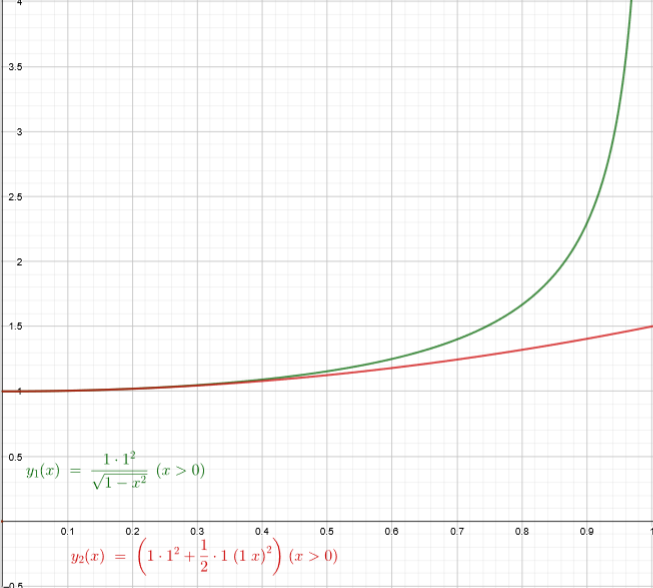
\includegraphics[width=0.6\linewidth]{energy.png}
    \caption{Comparison of relativistic energy and classical energy, dimensionless with $m = 1$, $c = 1$, and the horizontal axis is $\beta$.}
    \label{energy}
\end{figure}

In summary, various methods for handling Mass-Spring systems are relativistically modified, with the semi-implicit method being perfectly feasible. The implicit method has theoretical issues, but since it is not strictly enforced, calculations can still be performed step by step. The acceleration method does not provide any acceleration benefits. It can be anticipated that if the relativistic effects in a scene are strong, the time step requirements will be high, and there will be a tendency for energy explosion. The simulations below use the default object parameters: \lstinline|k = 1000, damping = 0.995, g = -9.8, collision penalty = 10000, collision scale factor = 1.1|. If the time step is set to 0.0001 and the speed of light is 100, decent results can be obtained over a period of time, although there is significant jitter. However, if the time step is set to 0.001 and the speed of light is 10, incorrect solutions will emerge midway, causing the grid results to disappear, as seen in \lstinline|cloth_semi_rela_0_10_0.001.gif| and \lstinline|cloth_semi_rela_0_100_0.0001.gif|. It can be proven that relativistic energy $\epsilon = \gamma mc^2$ is strictly greater than the classical kinetic energy plus rest energy $mc^2 + \frac{1}{2} mv^2$, and relativistic energy increases sharply with speed as the velocity approaches the speed of light, as shown in Figure \ref{energy}. This is also the reason why objects struggle to accelerate to the speed of light. However, the aforementioned simulation process is based on displacement and velocity, and when the velocity approaches the order of magnitude of the speed of light, energy increases sharply, requiring appropriate energy conservation corrections.

For the semi-implicit method, we directly calculate the acceleration, which then modifies velocity and position. Let the total energy at the $n$-th time step be $E_n = \sum \frac{1}{2} k (||\vec{x}_1 - \vec{x}_2|| - L)^2 + \sum (\gamma m c^2 - \vec{f}_{\text{ext}} \cdot \vec{x})$, and the total energy at the $n+1$-th time step be $E_{n+1}$. We consider a geometric decrease in the calculated acceleration. In actual simulation, $\vec{x}$ is finite because $\vec{v}$ is finite. After the approximation correction, the position $\vec{x}$ remains unchanged, and the increase in energy $\Delta E$ comes from changes in velocity $\vec{v}$ and potential energy. Using the new positions, we calculate the new potential energy, and from energy conservation, we get the kinetic energy and the required change in kinetic energy $\Delta E$:
$$ \Delta E = \sum \Delta(\gamma) m c^2 = \sum \frac{\vec{\beta} \cdot \mathrm{d} \vec{\beta}} {(1 - \beta^2)^{\frac{3}{2}}} mc^2 = \sum \frac{\vec{\beta} \cdot \vec{a} \mathrm{d} t} {(1 - \beta^2)^{\frac{3}{2}}} mc $$
Using the current calculated acceleration, we compute the result on the right side of the equation and compare it with the expected change in kinetic energy, which will give us the proportion by which the acceleration should be reduced.

This algorithm actually uses the tangent from Figure \ref{energy} for estimation. From the curve, it is apparent that when reaching the same energy, the velocity corresponding to the tangent will be greater than the true value. Additionally, by using the direct calculation of $\vec{x}$ as the potential energy estimate, in many cases, the kinetic energy will have excess room, causing energy to keep increasing. The actual situation is similar, and an explosion phenomenon might still occur. Considering the curve's properties, we can also perform secant estimation, i.e., calculate the next step's kinetic energy and adjust the energy difference by linear transformation to reach the target value. Similarly, we can analyze that the velocity at this time is underestimated, and combined with the large kinetic energy difference, the relationship between actual energy and original energy is uncertain, but the discrepancy is small, achieving stable energy. It should be noted that the energy we calculate is the sum of all particle energies, and does not follow a simple curve relationship. Furthermore, accelerations at different points do not necessarily increase velocity, so monotonicity of energy cannot be guaranteed. The above method also cannot guarantee that the kinetic energy will necessarily decrease or remain within a limited range. We should not simply apply linear changes because in certain specific situations, the computed energy difference may differ significantly from the target, which could be a sign of explosion.

If we take the ratio of the available kinetic energy increment to the current kinetic energy increment as the proportion, and truncate it to 1 when the absolute value exceeds 1, we will observe that when performing semi-implicit method simulations, at smaller speeds of light, the energy remains almost constant during the first swing of the cloth, resulting in good performance. However, when the swing reaches the peak, the available kinetic energy increment is positive while the current kinetic energy increment is negative. In this case, the speed should decrease according to the acceleration, but the above correction causes the acceleration to reverse, which does not match real motion. No matter how much the time step is reduced, the explosion phenomenon cannot be stopped, as seen in \lstinline|cloth_semi_rela_1_10_0.0001.gif| and \lstinline|cloth_semi_rela_1_100_0.0001.gif|. Therefore, in the correction process, we should ensure that energy does not increase, and handle the cases where the current kinetic energy increment is positive or negative separately. The final energy correction method we propose is as follows: for the cases where kinetic energy decreases or remains unchanged, we do not alter the calculated results, even if the potential energy demands further reduction of kinetic energy. For cases where kinetic energy increases, if potential energy requires a reduction, we set the acceleration to 0, since physically, the direction of the velocity should not change; if potential energy demands an increase in kinetic energy, we process it proportionally, ensuring it does not exceed 1. This method cannot strictly guarantee that energy will not increase (even the previously described methods cannot fully guarantee this due to potential energy uncertainties and the superposition of multiple particles), but in practice, the energy changes are small each time, and overall energy is approximately conserved. However, due to the inherent instability of the semi-implicit method, explosions still occur after long simulation times, and this phenomenon cannot be corrected using the energy correction method mentioned above, as the direction of the velocity is already incorrect, causing the grid to continuously expand in the wrong direction, as seen in \lstinline|cloth_semi_rela_2_10_0.0005.gif| and \lstinline|cloth_semi_rela_2_100_0.001.gif|. To achieve more accurate results, the time step must be reduced continuously.

For the implicit method, theoretically, a larger time step can be used. Similar energy correction methods can be applied, but the acceleration involved should be modified to $a = \frac{\Delta \vec{x} /h - \vec{v}} {h}$. In the implicit method, solving $(\mathbf{I} - \vec{\beta} \vec{\beta}^{T}) \mathbf{He}$ requires attention to avoid using the multiplication provided by \lstinline|Eigen::MatrixXd|, as unexpected results with very large numbers can occur. It is best to use the matrix multiplication definition, and since the matrix is only $3 \times 3$, it does not affect the running efficiency and ensures the correctness of the result. Without energy correction, the simulation will exhibit explosion phenomena, represented by the matrix's minimum eigenvalue gradually decreasing to below 0, after which the equation becomes unsolvable and explodes after positive definiteness. If tangent-based energy corrections are applied, the results are similar to those without correction but still exhibit significant explosions. The secant estimation correction method yields the best results, with no explosions. See \lstinline|cloth_imp_rela_0_10_0.001.gif|, \lstinline|cloth_imp_rela_1_10_0.001.gif|, \lstinline|cloth_imp_rela_2_10_0.001.gif| for details. The secant method also works well for simulating very low light speeds, as seen in \lstinline|cloth_imp_rela_2_1_0.001.gif|.

Non-relativistic simulation results are given in \lstinline|cloth_semi_0.001.gif| and \lstinline|cloth_imp_0.001.gif|. In general, the semi-implicit method shows larger, more dramatic energy changes, with the relativistic and non-relativistic cases not differing significantly. The implicit method shows slightly smaller and less fluctuating energy, with relativistic effects becoming more pronounced at lower speeds of light, making acceleration more difficult. However, the secant energy correction algorithm will gradually reduce energy, giving the effect of damping. Theoretically, as long as a sufficiently small time step is chosen, both the secant-corrected implicit and semi-implicit methods can achieve better simulation results.

In this framework, collision penalty forces can also be used to simulate cloth-object collisions, as seen in \\ \lstinline|cloth_ball_imp_rela_2_10_0.001.gif| and \lstinline|cloth_ball_imp_rela_2_10_0.001_2.gif|. Other spring-particle type object motions, such as simulating a collision between an elastic and a rigid ball, can also be modeled, as seen in \\ \lstinline|ball_ball_imp_rela_2_10_0.001.gif|.

The correction methods can be refined further. Tangent and secant corrections are approximations using tangents and secants, respectively. In reality, we can model the decay proportion as a function, and the problem becomes finding the zero point of the function that achieves the desired energy difference. This is a root-finding problem that can be solved using methods like binary search or Newton's method. It is important to note that due to the presence of multiple particles, the function's shape and monotonicity are uncertain, and precautions should be taken to ensure the results stay within a reasonable range, with the results from tangent and secant corrections serving as boundaries.

In principle, we can use the relativistic dynamics equations to perform more systematic physical simulations, including fluid simulations. Given the relationship between relativistic energy and velocity, a very small time step is required for good simulation when the speed of light is low, and appropriate energy conservation correction algorithms need to be added. For physical simulations at low light speeds, new algorithms should be developed from the perspective of energy as an independent variable to balance time and effectiveness.

\subsubsection*{Trade-offs and Improvements in Rendering}

When the speed of light is low enough to compare with the speed of an object, the geometry of the object in the observer's view will be distorted not only due to the time it takes for light to propagate but also its shadows. As mentioned earlier, the geometric distortion can be solved using Newton's iteration method to find the zero point of a function, providing a physically accurate result. However, for shadows, the changes in geometry are much more complex. To determine whether a fragment is in the shadow of a light source, we need to check if the light from the source is obstructed by the moving object as it travels toward the fragment. A simple idea is to apply a time delay to the vertex transformation of the light source, similar to the observer’s perspective, and then calculate the corresponding Shadow Map. However, the downside of this approach is that the light also takes time to travel from the fragment to the observer. This means that each fragment would need to fetch the Shadow Map corresponding to its \(t^{*}\) moment to determine whether it is in shadow, which is still unrealistic for shaders.

Considering that this project is a demonstration of relativistic visual simulation rather than a pursuit of accurate shadows, we made a trade-off in the handling of shadows: we do not compute shadowing based on the light source but instead use Blinn-Phong lighting combined with SSAO to render lighting and shadow effects. To make this rendering effect more convincing, the demonstration scene in this project uses only a single high-position point light, making ambient occlusion the main component of scene shadows, resulting in a visually pleasing effect.

For better visual quality, we further improved the Render Node system. Considering possible post-processing requirements, we added a Post Process node that takes information from the G-Buffer and four custom parameters and passes them to a fragment shader, which can be written freely. This node is an extension of the original SSAO node and, while maintaining compatibility with SSAO shaders, also allows the calling of other shaders to implement additional post-processing effects. For example, we wrote a bilateral filter (Bilateral Filter) shader to denoise the results generated by SSAO; the skybox in the test scene is also calculated in the post-processing shader \lstinline|relativity_background.fs|. Common post-processing effects such as blur, hue shifts, and bloom can also be easily implemented within this framework, although they were not applied in this project.

We also created a Mix Color post-processing node. This node implements a custom image blending mode by passing two images and an alpha parameter into the fragment shader, enabling various effects. For instance, the SSAO node does not need to pass the original image but instead outputs only the pure AO result. This result can then be merged with the deferred lighting output using the multiply mode. This new workflow allows the pure AO result to be denoised through bilateral filtering before being applied to the original image. Additionally, by blending the results from relativistic rasterization and traditional rasterization using transparency modes, we can compare the positions of objects in the original and relativistic-transformed space on the same screen, with excellent results.

Considering that all objects in the main test scene use a checkerboard texture, we switched the texture filtering mode to nearest-neighbor interpolation, avoiding the blurring caused by linear interpolation of the checkerboard texture. This resulted in sharper edges and significantly improved the visual effect.

A complete rendering node graph is shown in Figure \ref{render}.

\begin{figure}[htbp]
    \centering
    \setlength{\abovecaptionskip}{0.cm}
    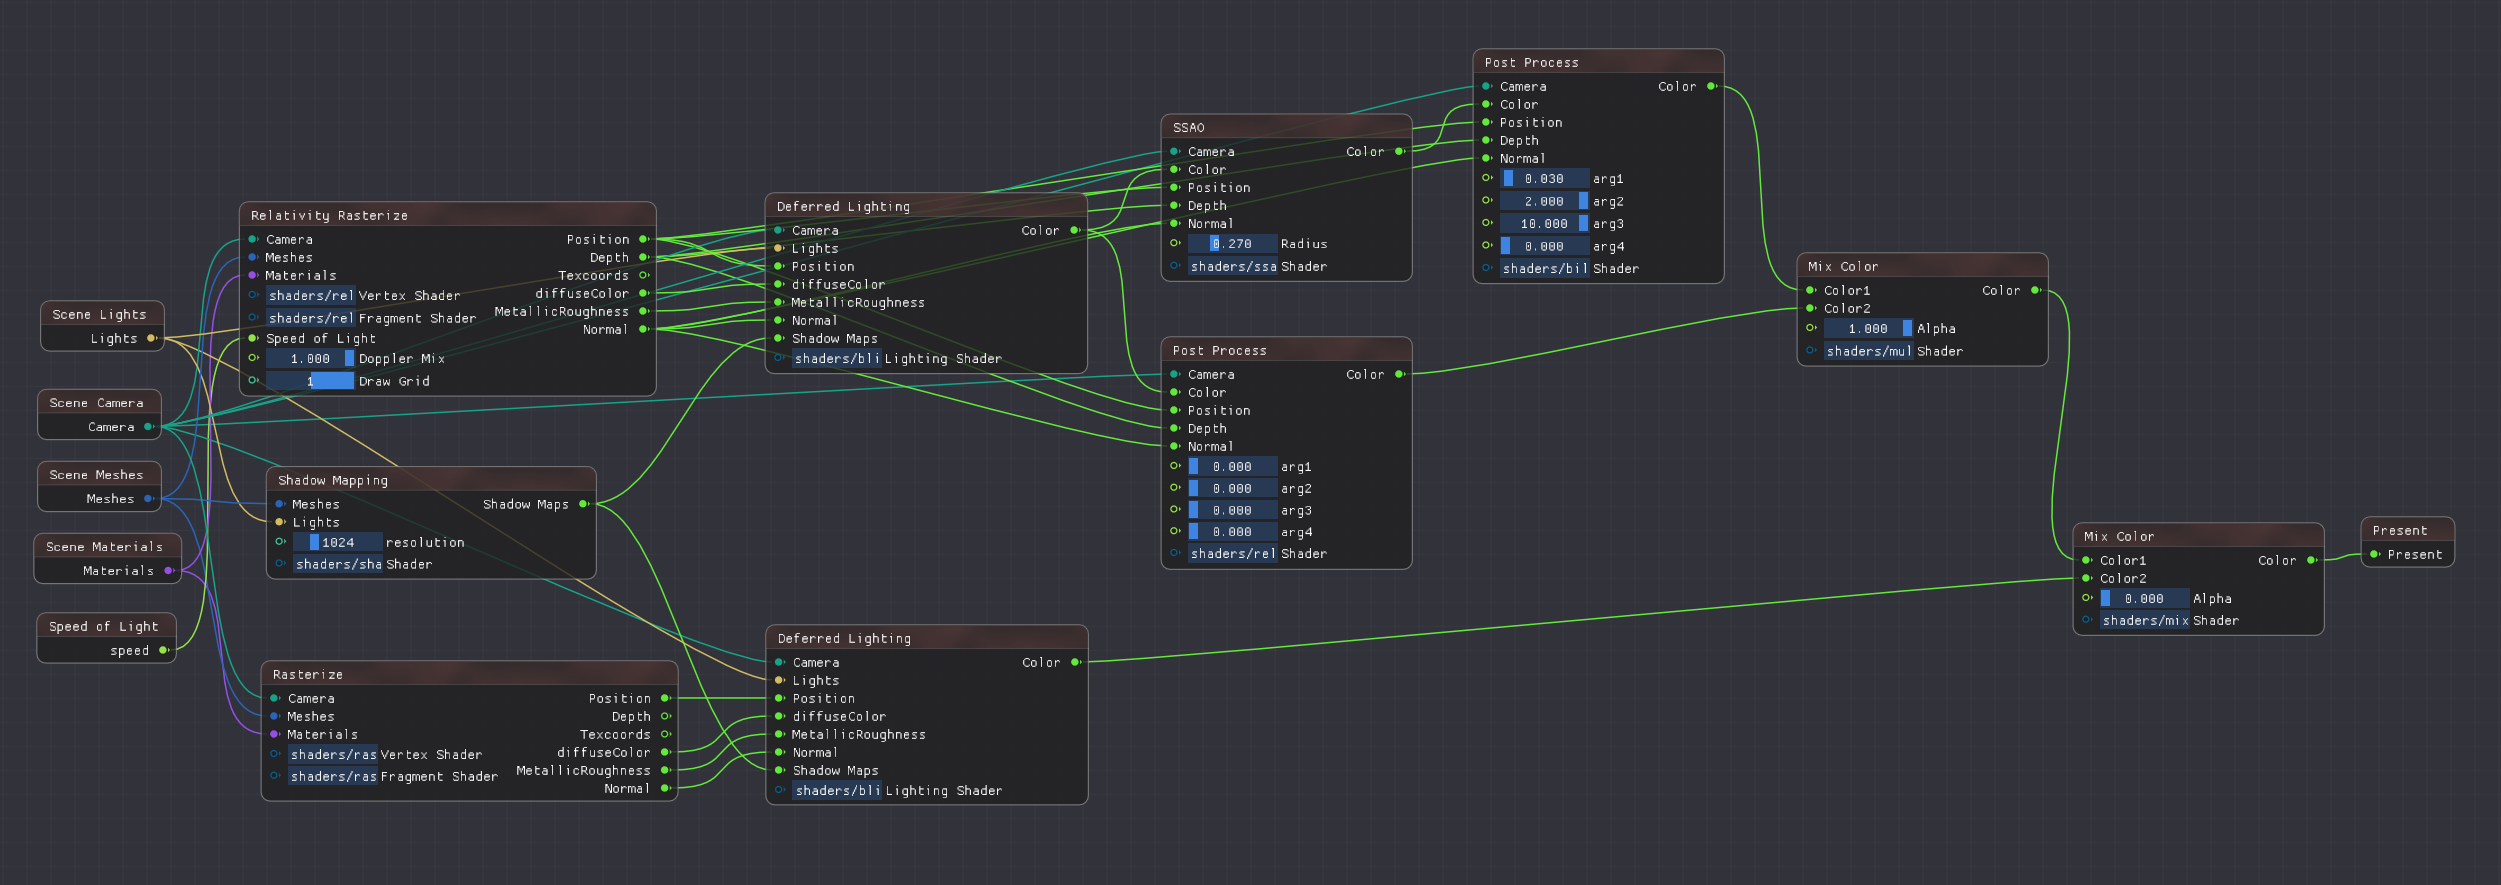
\includegraphics[width=\linewidth]{RenderGraph.png}
    \caption{Complete rendering node graph}
    \label{render}
\end{figure}

\subsubsection*{Scene Setup}

The main test scene in this project is largely inspired by the video "Relativistic Visual Effects Misunderstood by Einstein" (\url{https://www.bilibili.com/video/BV1JY411L7xm}). Inspired by this video, the test scene in this project uses checkerboard textures on objects to observe the geometric distortion under relativistic effects. Additionally, we created models of moving cubes, rotating spheres, and other models similar to those in the video using Blender, to test the relativistic distortions of objects and the Doppler effect.

To provide good positional reference, a \(5\text{m} \times 5\text{m}\) checkerboard floor was laid out in the test scene. This floor is also involved in the calculation of relativistic distortions to avoid mesh clipping. Furthermore, in the relativistic rasterization node, an OpenGL interface is used to draw a set of ground meshes that are not affected by relativistic transformations, allowing for a clearer observation of the degree of geometric distortion.

In this project, all relativistic distortions are applied to vertex transformations. As a result, meshes with sparse vertices will not properly exhibit the "twisting" effect and may result in clipping when interacting with other objects. This means that all curved surfaces in the test scene need to be sufficiently subdivided. The floor and cubes in the main test scene are high-poly models that were pre-subdivided. Additionally, the walls and floors in the \lstinline|Sponza.usda| model were further subdivided using Blender to create the \lstinline|Sponza_subdivided.usda| model to meet the requirements of geometric transformation.

To avoid the scene feeling too monotonous, a gradient skybox was added through post-processing. When objects are farther away in the scene, their colors blend with the skybox to create a fog effect, making the visual effect of the ground mesh more natural.

\subsection*{4\quad Project Summary}

In this project, we successfully achieved the following:
\begin{enumerate}[(1)]
    \item Simulated relativistic visual effects in static scenes;
    \item Simulated relativistic visual effects in dynamic scenes with delayed equation solving, achieving nearly real-time effects and forming a complete relativistic visual simulation method;
    \item Simulated an "overhead" view;
    \item Simulated relativistic dynamics of a particle-spring system.
\end{enumerate}

However, there are still several shortcomings in this project, such as:
\begin{enumerate}[(1)]
    \item The camera reference frame is an "instantaneous comoving" frame, meaning that if the object has high acceleration, special relativity no longer applies;
    \item We did not distinguish between the camera's proper time and the default system time;
    \item We cannot handle the creation or disappearance of objects, as this involves changes in mesh topology;
    \item The rasterization result is affected by mesh precision, making high-precision transformations difficult to achieve;
    \item The color changes due to Doppler shift are not physically accurate; they are simply a result of a linear approximation;
    \item The overhead view simulation process is not user-friendly and requires additional operations;
    \item The energy conservation correction in the particle-spring system physics simulation is not precise enough, and we cannot ensure that energy changes remain within a reasonable range.
\end{enumerate}

Through the practice of this project, we gained a deeper understanding of special relativity and a more intuitive experience of visual effects under special relativity. At the same time, we further consolidated and applied many concepts learned in the computer graphics course and gained a basic understanding of how a node-based rendering framework operates. We also gained greater clarity on the overall process of a large-scale project. During the project, we encountered many difficulties, such as understanding the operation of the framework, theoretical challenges with the overhead view, energy conservation issues in physics simulation, and the trade-offs in rendering. Solving these problems expanded our thinking and helped us learn more.

\subsection*{5\quad Acknowledgments}

We would like to thank the teaching assistants Pengfei Shen, Zhehao Li, and Wenzheng Wu from the computer graphics course for providing the framework support for this project and offering careful guidance on modifications to the framework. Special thanks to Assistant Pengfei Shen for offline assistance in implementing the feature to retrieve the history of node positions.

We also thank the MIT Game Lab for creating the game *A Slower Speed of Light*, which provided a reference for the expected effects of geometric distortion and Doppler effects; and we thank Bilibili user "Two Ripe Plums" for creating the series of videos on relativistic visual effects, which inspired the design of the test scene and the expected display effects.

\label{unknown}
\end{document}